\documentclass{beamer}
\usetheme{Warsaw}
\usepackage{natbib}
\usepackage{graphicx}
% ------------------------------------------------------------------------
% Packages
% ------------------------------------------------------------------------
\usepackage{amsmath}

% ------------------------------------------------------------------------
% Macros
% ------------------------------------------------------------------------
%~~~~~~~~~~~~~~~
% List shorthand
%~~~~~~~~~~~~~~~
\newcommand{\BIT}{\begin{itemize}}
\newcommand{\EIT}{\end{itemize}}
\newcommand{\BNUM}{\begin{enumerate}}
\newcommand{\ENUM}{\end{enumerate}}
%~~~~~~~~~~~~~~~
% Text with quads around it
%~~~~~~~~~~~~~~~
\newcommand{\qtext}[1]{\quad\text{#1}\quad}
%~~~~~~~~~~~~~~~
% Shorthand for math formatting
%~~~~~~~~~~~~~~~
\newcommand\mbb[1]{\mathbb{#1}}
\newcommand\mbf[1]{\mathbf{#1}}
\def\mc#1{\mathcal{#1}}
\def\mrm#1{\mathrm{#1}}
%~~~~~~~~~~~~~~~
% Common sets
%~~~~~~~~~~~~~~~
\def\reals{\mathbb{R}} % Real number symbol
\def\integers{\mathbb{Z}} % Integer symbol
\def\rationals{\mathbb{Q}} % Rational numbers
\def\naturals{\mathbb{N}} % Natural numbers
\def\complex{\mathbb{C}} % Complex numbers
\def\simplex{\mathcal{S}} % Simplex
%~~~~~~~~~~~~~~~
% Common functions
%~~~~~~~~~~~~~~~
\renewcommand{\exp}[1]{\operatorname{exp}\left(#1\right)} % Exponential
\def\indic#1{\mbb{I}\left({#1}\right)} % Indicator function
\providecommand{\argmax}{\mathop\mathrm{arg max}} % Defining math symbols
\providecommand{\argmin}{\mathop\mathrm{arg min}}
\providecommand{\arccos}{\mathop\mathrm{arccos}}
\providecommand{\asinh}{\mathop\mathrm{asinh}}
\providecommand{\dom}{\mathop\mathrm{dom}} % Domain
\providecommand{\range}{\mathop\mathrm{range}} % Range
\providecommand{\diag}{\mathop\mathrm{diag}}
\providecommand{\tr}{\mathop\mathrm{tr}}
\providecommand{\abs}{\mathop\mathrm{abs}}
\providecommand{\card}{\mathop\mathrm{card}}
\providecommand{\sign}{\mathop\mathrm{sign}}
\def\rank#1{\mathrm{rank}({#1})}
\def\supp#1{\mathrm{supp}({#1})}
%~~~~~~~~~~~~~~~
% Common probability symbols
%~~~~~~~~~~~~~~~
\def\E{\mathbb{E}} % Expectation symbol
\def\Earg#1{\E\left[{#1}\right]}
\def\Esubarg#1#2{\E_{#1}\left[{#2}\right]}
\def\P{\mathbb{P}} % Probability symbol
\def\Parg#1{\P\left({#1}\right)}
\def\Psubarg#1#2{\P_{#1}\left[{#2}\right]}
\def\Cov{\mrm{Cov}} % Covariance symbol
\def\Covarg#1{\Cov\left[{#1}\right]}
\def\Covsubarg#1#2{\Cov_{#1}\left[{#2}\right]}
\def\Var{\mrm{Var}}
\def\Vararg#1{\Var\left(#1\right)}
\def\Varsubarg#1#2{\Var_{#1}\left(#2\right)}
\newcommand{\family}{\mathcal{P}} % probability family
\newcommand{\eps}{\epsilon}
\def\absarg#1{\left|#1\right|}
\def\msarg#1{\left(#1\right)^{2}}
\def\logarg#1{\log\left(#1\right)}
%~~~~~~~~~~~~~~~
% Distributions
%~~~~~~~~~~~~~~~
\def\Gsn{\mathcal{N}}
\def\Ber{\textnormal{Ber}}
\def\Bin{\textnormal{Bin}}
\def\Unif{\textnormal{Unif}}
\def\Mult{\textnormal{Mult}}
\def\Cat{\textnormal{Cat}}
\def\Gam{\textnormal{Gam}}
\def\InvGam{\textnormal{InvGam}}
\def\NegMult{\textnormal{NegMult}}
\def\Dir{\textnormal{Dir}}
\def\Lap{\textnormal{Laplace}}
\def\Bet{\textnormal{Beta}}
\def\Poi{\textnormal{Poi}}
\def\HypGeo{\textnormal{HypGeo}}
\def\GEM{\textnormal{GEM}}
\def\BP{\textnormal{BP}}
\def\DP{\textnormal{DP}}
\def\BeP{\textnormal{BeP}}
%~~~~~~~~~~~~~~~
% Theorem-like environments
%~~~~~~~~~~~~~~~

%-----------------------
% Probability sets
%-----------------------
\newcommand{\X}{\mathcal{X}}
\newcommand{\Y}{\mathcal{Y}}
\newcommand{\D}{\mathcal{D}}
\newcommand{\Scal}{\mathcal{S}}
%-----------------------
% vector notation
%-----------------------
\newcommand{\bx}{\mathbf{x}}
\newcommand{\by}{\mathbf{y}}
\newcommand{\bt}{\mathbf{t}}
\newcommand{\xbar}{\overline{x}}
\newcommand{\Xbar}{\overline{X}}
\newcommand{\tolaw}{\xrightarrow{\mathcal{L}}}
\newcommand{\toprob}{\xrightarrow{\mathbb{P}}}
\newcommand{\laweq}{\overset{\mathcal{L}}{=}}
\newcommand{\F}{\mathcal{F}}
\def\colarg#1#2{\textcolor[HTML]{#1}{#2}}

\setbeamersize{text margin left=5pt,text margin right=5pt}

\setbeamerfont{institute}{size=\fontsize{7pt}{8pt}}
\setbeamerfont{date}{size=\fontsize{0pt}{0pt}}

\title{Methods for Regime Detection and Multitable Analysis}
\author{Kris Sankaran}

\begin{document}
\maketitle

\begin{frame}
  \frametitle{Problems of Interest}
 \begin{itemize}
 \item Regime Detection: Can we segment time intervals in a microbiome study in
   an unsupervised way?
   \begin{itemize}
   \item Intervals with similar dynamics should be placed in the same regime
   \item Can we characterize differences between taxa during these regimes?
   \end{itemize}
 \item Multitable Analysis: How should we simultaneously study multiple
   measurement types?
   \begin{itemize}
   \item How do different measurement types covary with one another?
   \item Compared to usual regression, when there are multiple related
     responses, there are fewer obvious practical approaches
   \end{itemize}
 \item Philosophy: Distill relevant themes, provide concrete workflows, and
   systematize data / study-specific recommendations
 \end{itemize}
\end{frame}

\section{Regime Detection}
\label{sec:regime_detection}

\begin{frame}
  \frametitle{Recap}
 \begin{itemize}
 \item For this case study, we again use the antibiotics data of
   \citep{dethlefsen2008pervasive}
   \begin{itemize}
   \item 3 subjects at between 52 and 56 timepoints
   \item Two antibiotic time courses introduced around 12 - 16 and 40 - 44
   \item Long term effects in Subject F previously observed
   \end{itemize}
 \item Last time we approached the regime detection problem using hierarchical
   clustering with various distances, HMMs, Sticky HMMs, Infinite HMMs, and
   Switching Dynamical Systems
 \item We continue that survey using different approaches
 \end{itemize}
\end{frame}

\subsection{CART}
\label{subsec:CART}

\begin{frame}
  \frametitle{CART}
  \begin{itemize}
  \item Order species according to a hierarchical
    clustering\footnote{Alternatively, use phylogenetic similarity.}, and
    consider the surface of species abundances across the time $\times$ species space
  \item CART can approximate this surface, providing a partition of timepoints
    and species in the process.
  \item Can be extended to binary data
  \item Limitation: Cannot update the species order (though you could imagine an
    iterative approach...)
  \end{itemize}
\end{frame}

\begin{frame}
  \frametitle{CART}
\begin{itemize}
\item Structural model: The class of functions $\mathcal{F}$ that can be
  expressed as
\begin{align*}
  f\left(x\right) &= \sum_{m = 1}^{M} c_{m} \indic{x \in R_{m}},
\end{align*}
\item Fitting criteria: Minimize the expected generalization squared-error,
\begin{align*}
  \frac{1}{n} \sum_{i = 1}^{n} \left(y_{i} - c\left(x_{i}\right)\right)^{2},
\end{align*}
\item Estimation strategy: Recursively split rectangles into left ($l$) and
  right ($r$) subrectangles according to
\begin{align*}
  \left(j^{\ast}, t_{j1}^{\ast}\right) &= \arg \min_{\substack{j = 1, \dots, p \\ t_{j1} \in \reals}} \sum_{i \in R_{1, l}} \left(y_{i} - \bar{y}_{l}\right)^{2} + \sum_{i \in R_{1, r}} \left(y_{i} - \bar{y}_{r}\right)^{2}
\end{align*}
and prune to prevent overfitting
\end{itemize}
\end{frame}

\begin{frame}
  \frametitle{CART ($\asinh$ abundance)}
  \begin{figure}[ht]
    \centering
    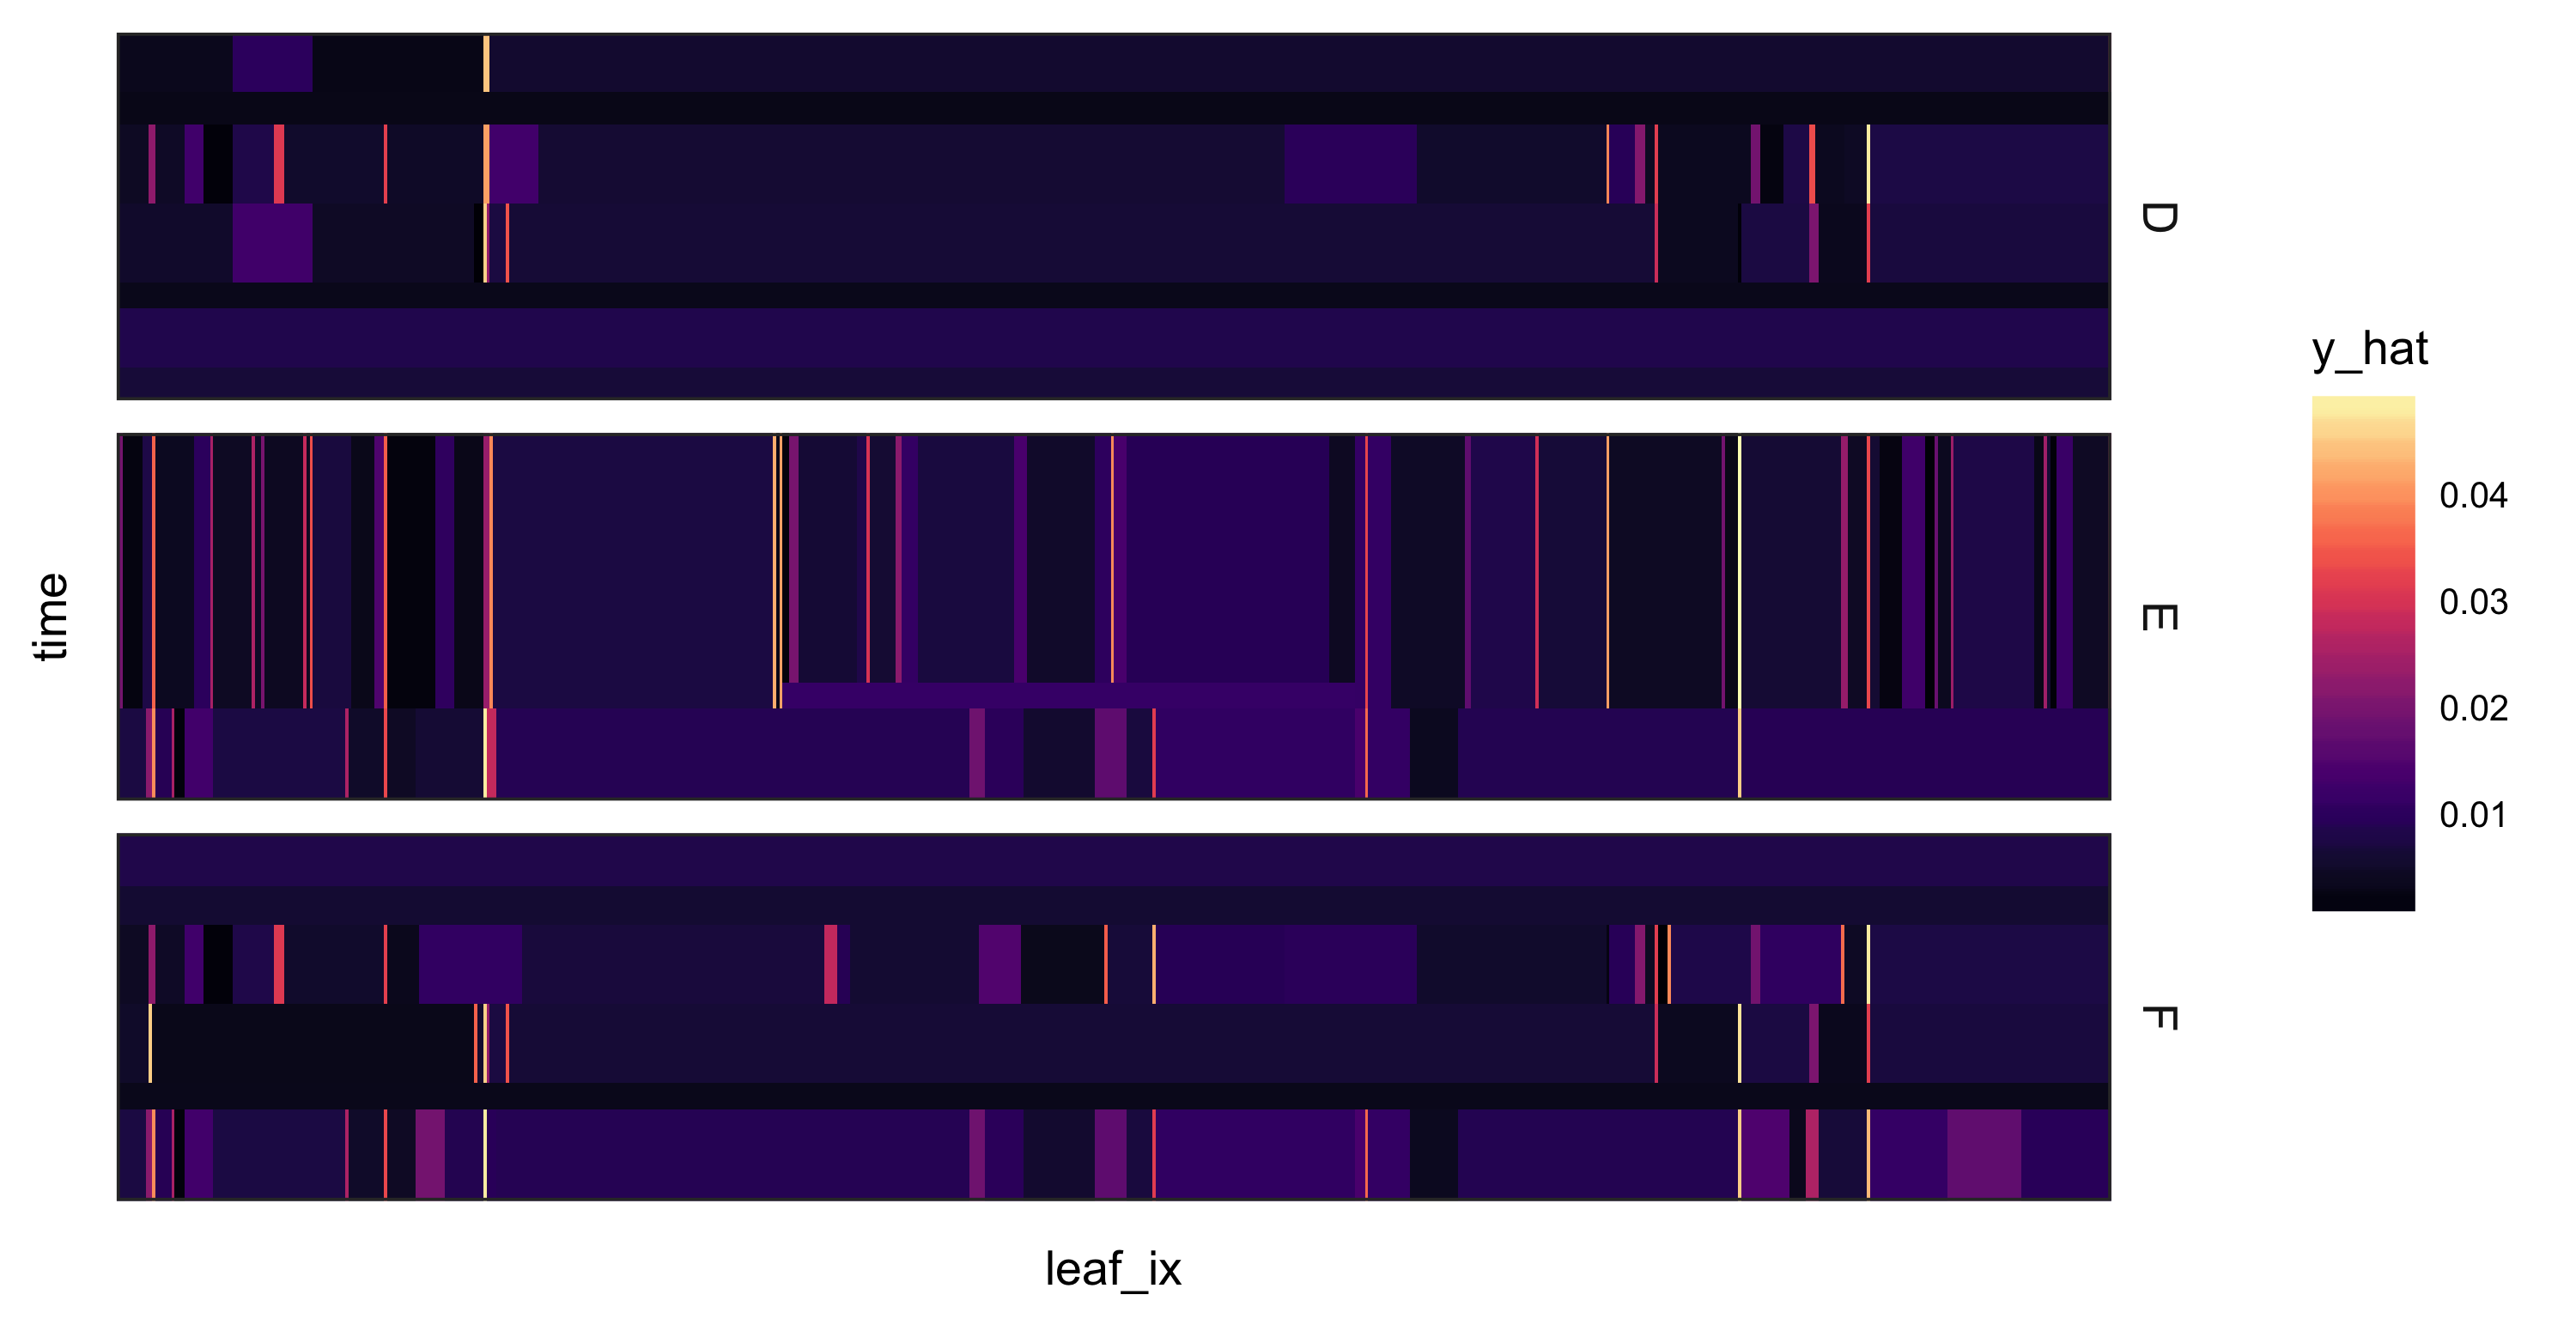
\includegraphics[width=.8\textwidth]{figure/rpart_complex_2}
    \caption{Each panel represents a subject, the $x$-axis are individual
      species, the $y$-axis indexes time, and the color is the predicted
      abundance according to CART. Note the low abundance predictions during the
      antibiotic time courses. \label{fig:rpart_complex} }
  \end{figure}
\end{frame}

\begin{frame}
  \frametitle{CART (Residual)}
  \begin{figure}[ht]
    \centering
    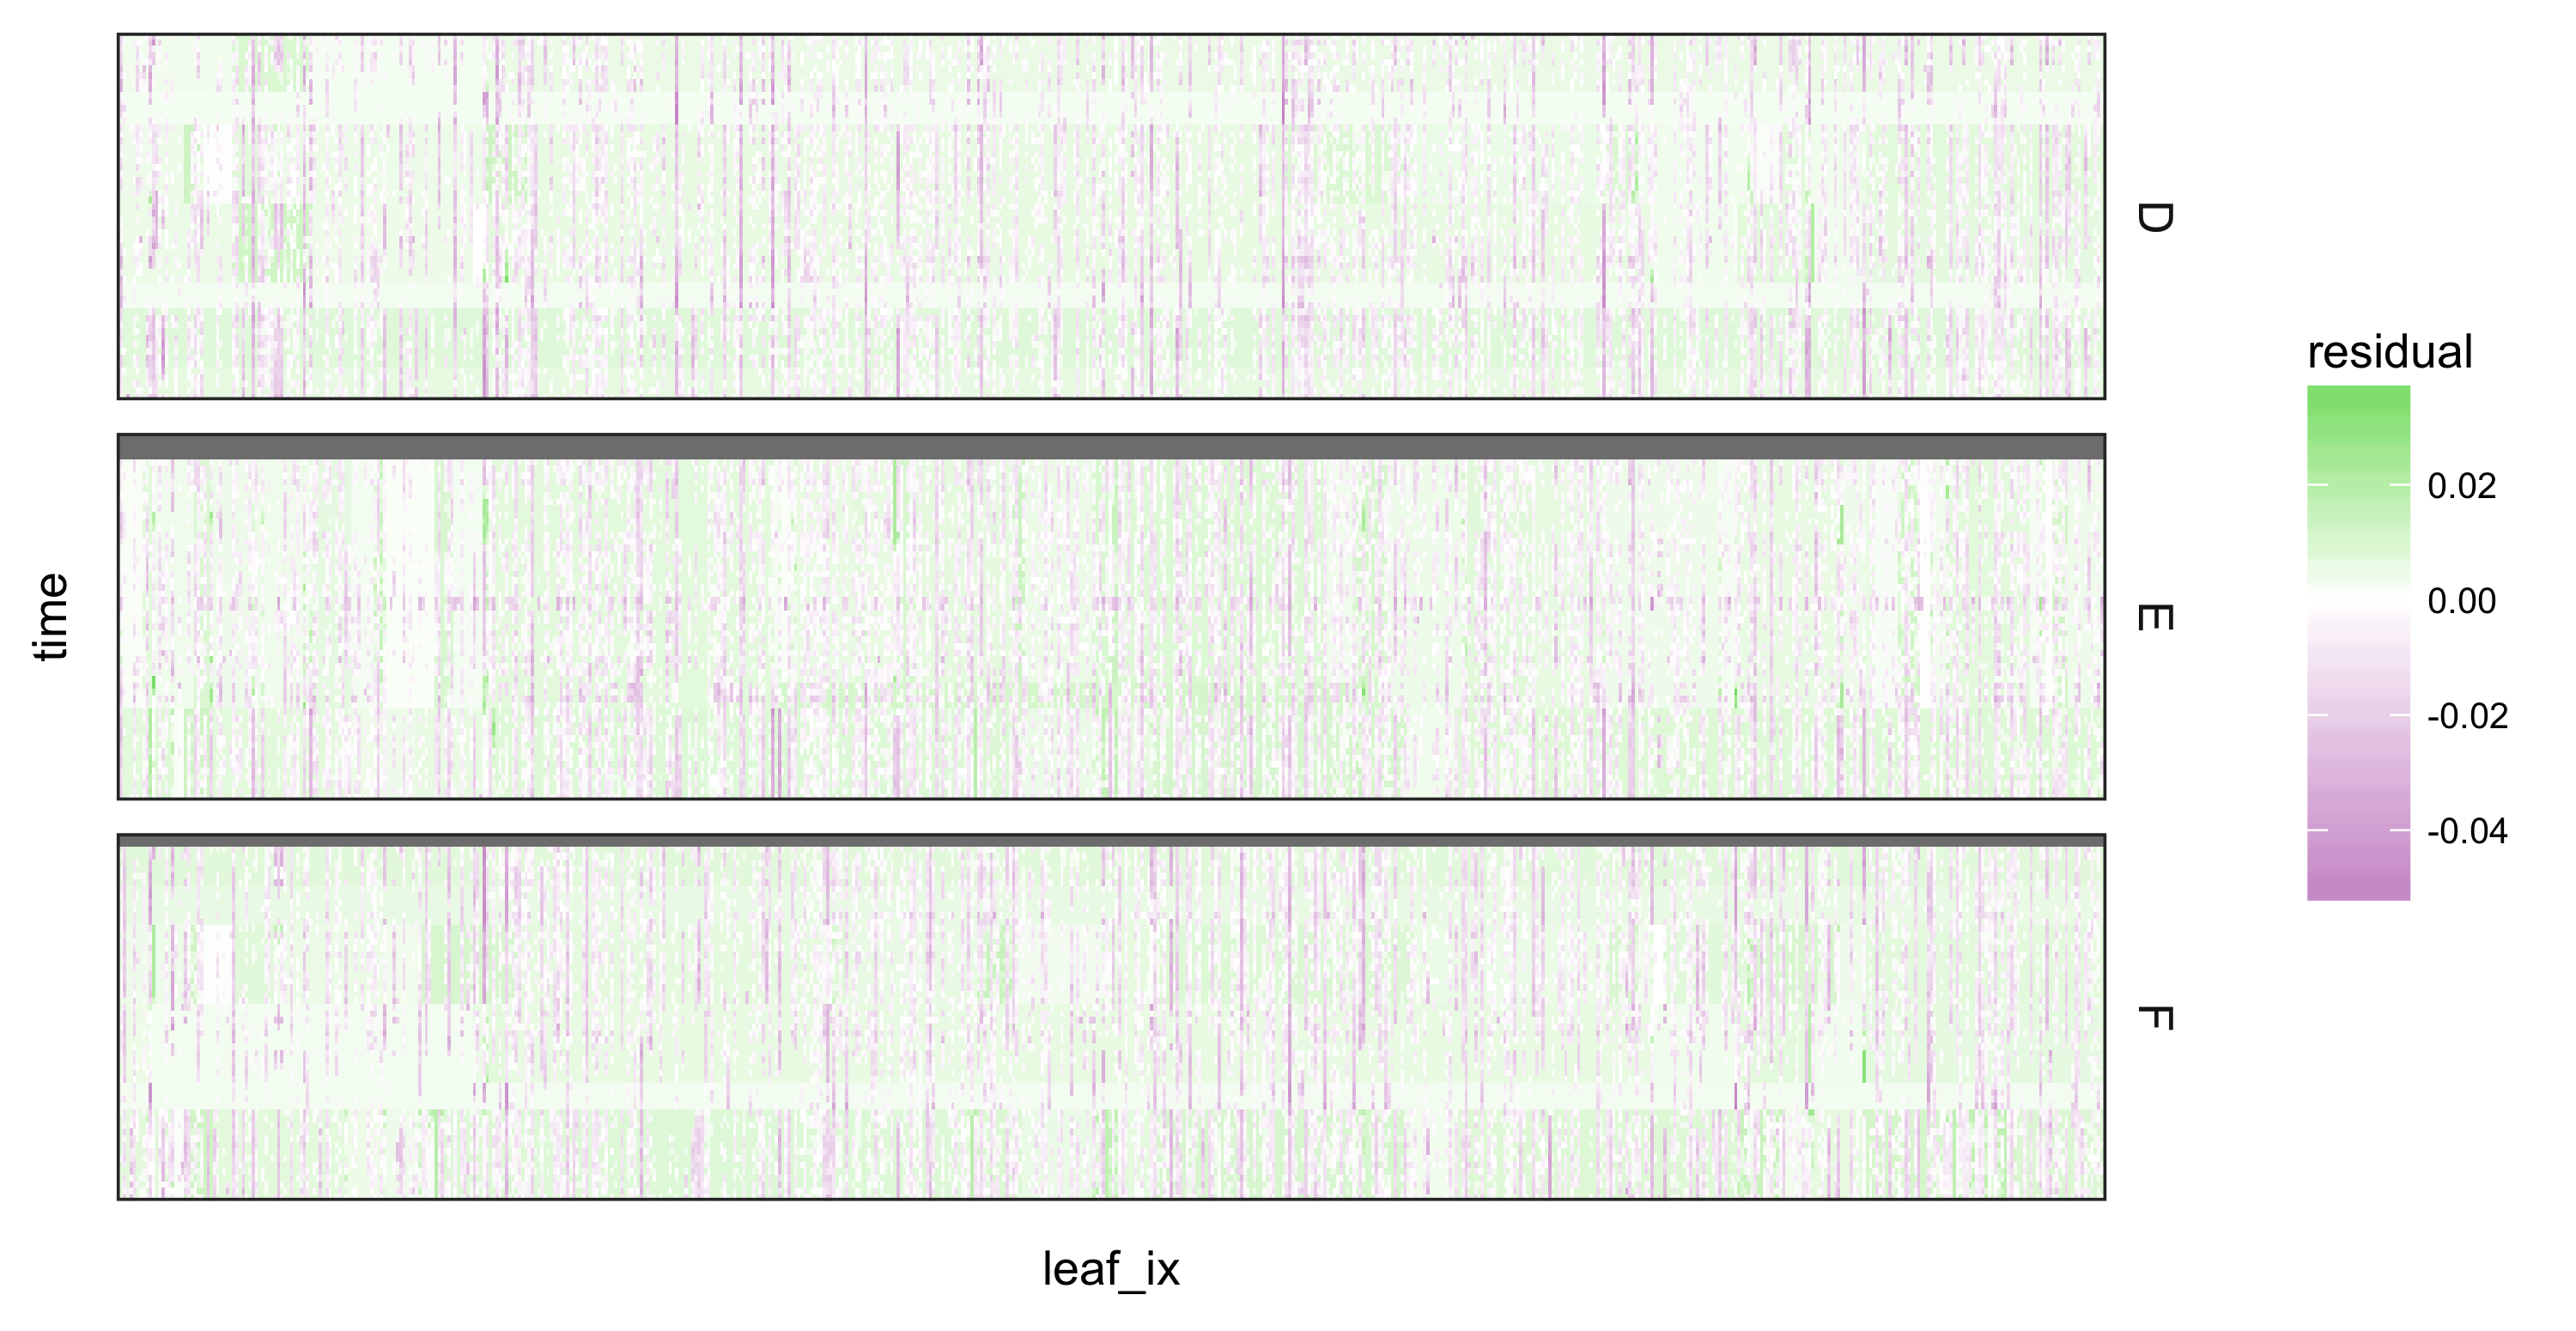
\includegraphics[width=.8\textwidth]{figure/rpart_complex_2_resid}
    \caption{An advantage of using a regression model is that we can directly
      inspect the quality of model fit, using
      residuals. \label{fig:rpart_complex_resid} }
  \end{figure}
\end{frame}

\begin{frame}
  \frametitle{Adjusting Model Complexity}
  \begin{figure}[ht]
    \centering
    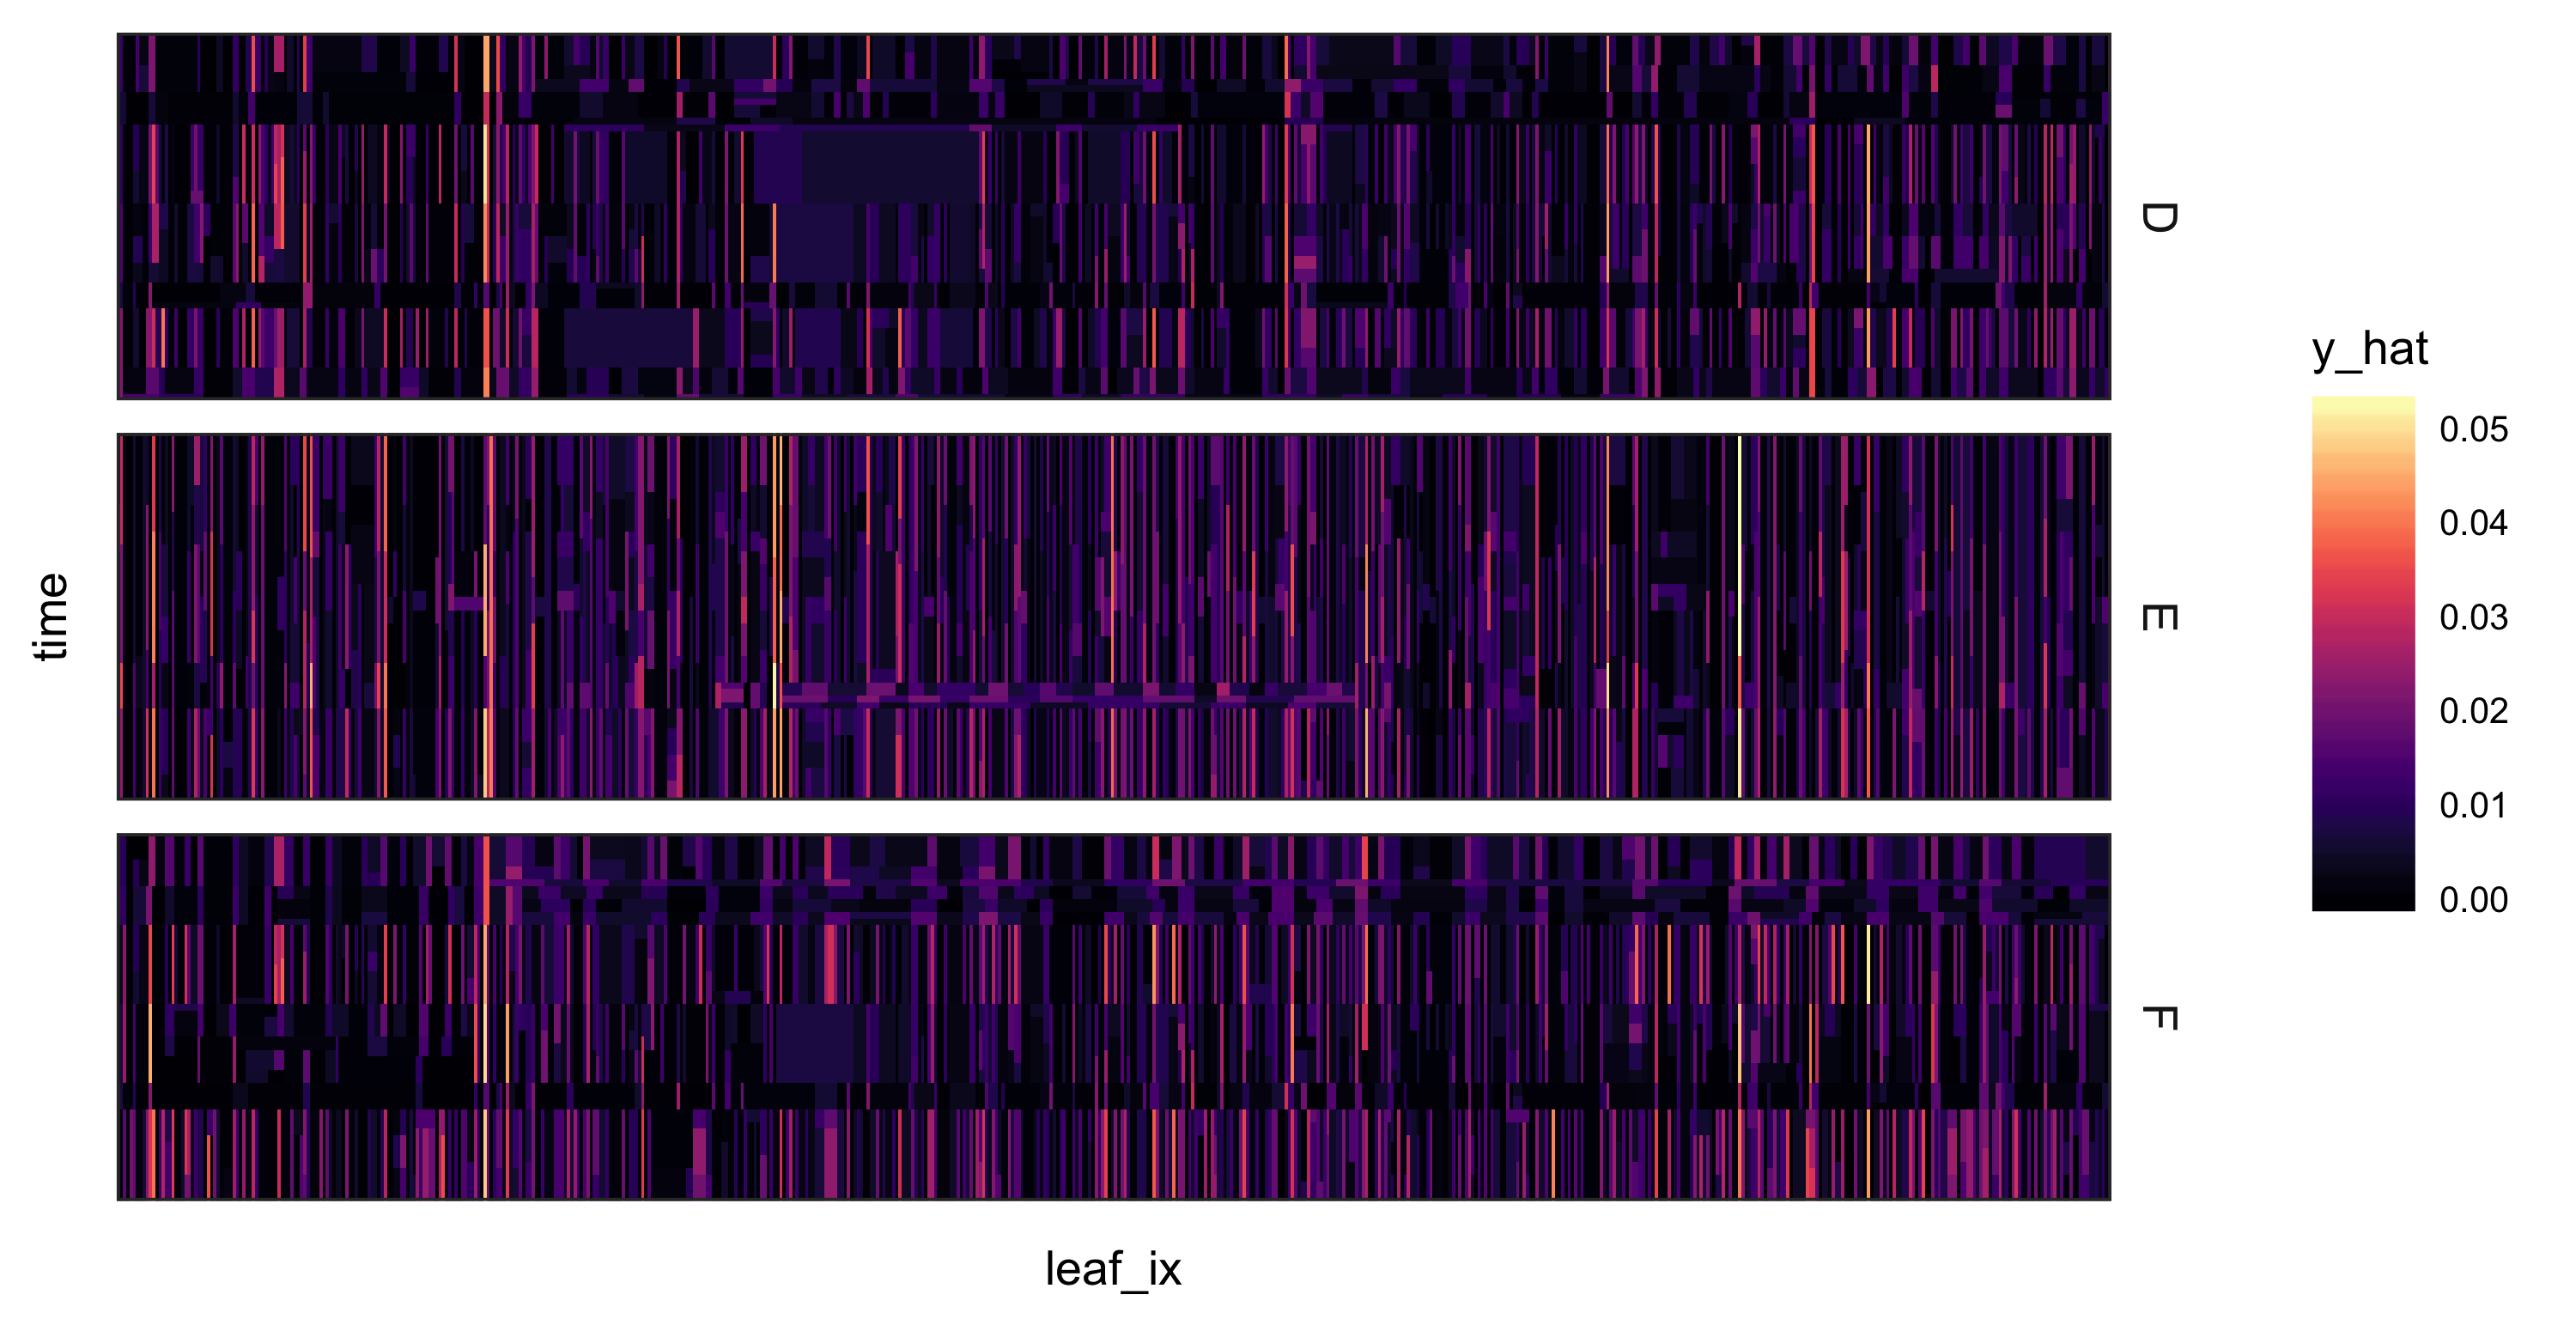
\includegraphics[width=.8\textwidth]{figure/rpart_simple}
    \caption{By increasing the model complexity, we notice species with
      increasing abundances during the antibiotic time
      courses. \label{fig:rpart_simple} }
  \end{figure}
\end{frame}

\begin{frame}
  \frametitle{CART (Presence / Absence)}
  \begin{figure}[ht]
    \centering
    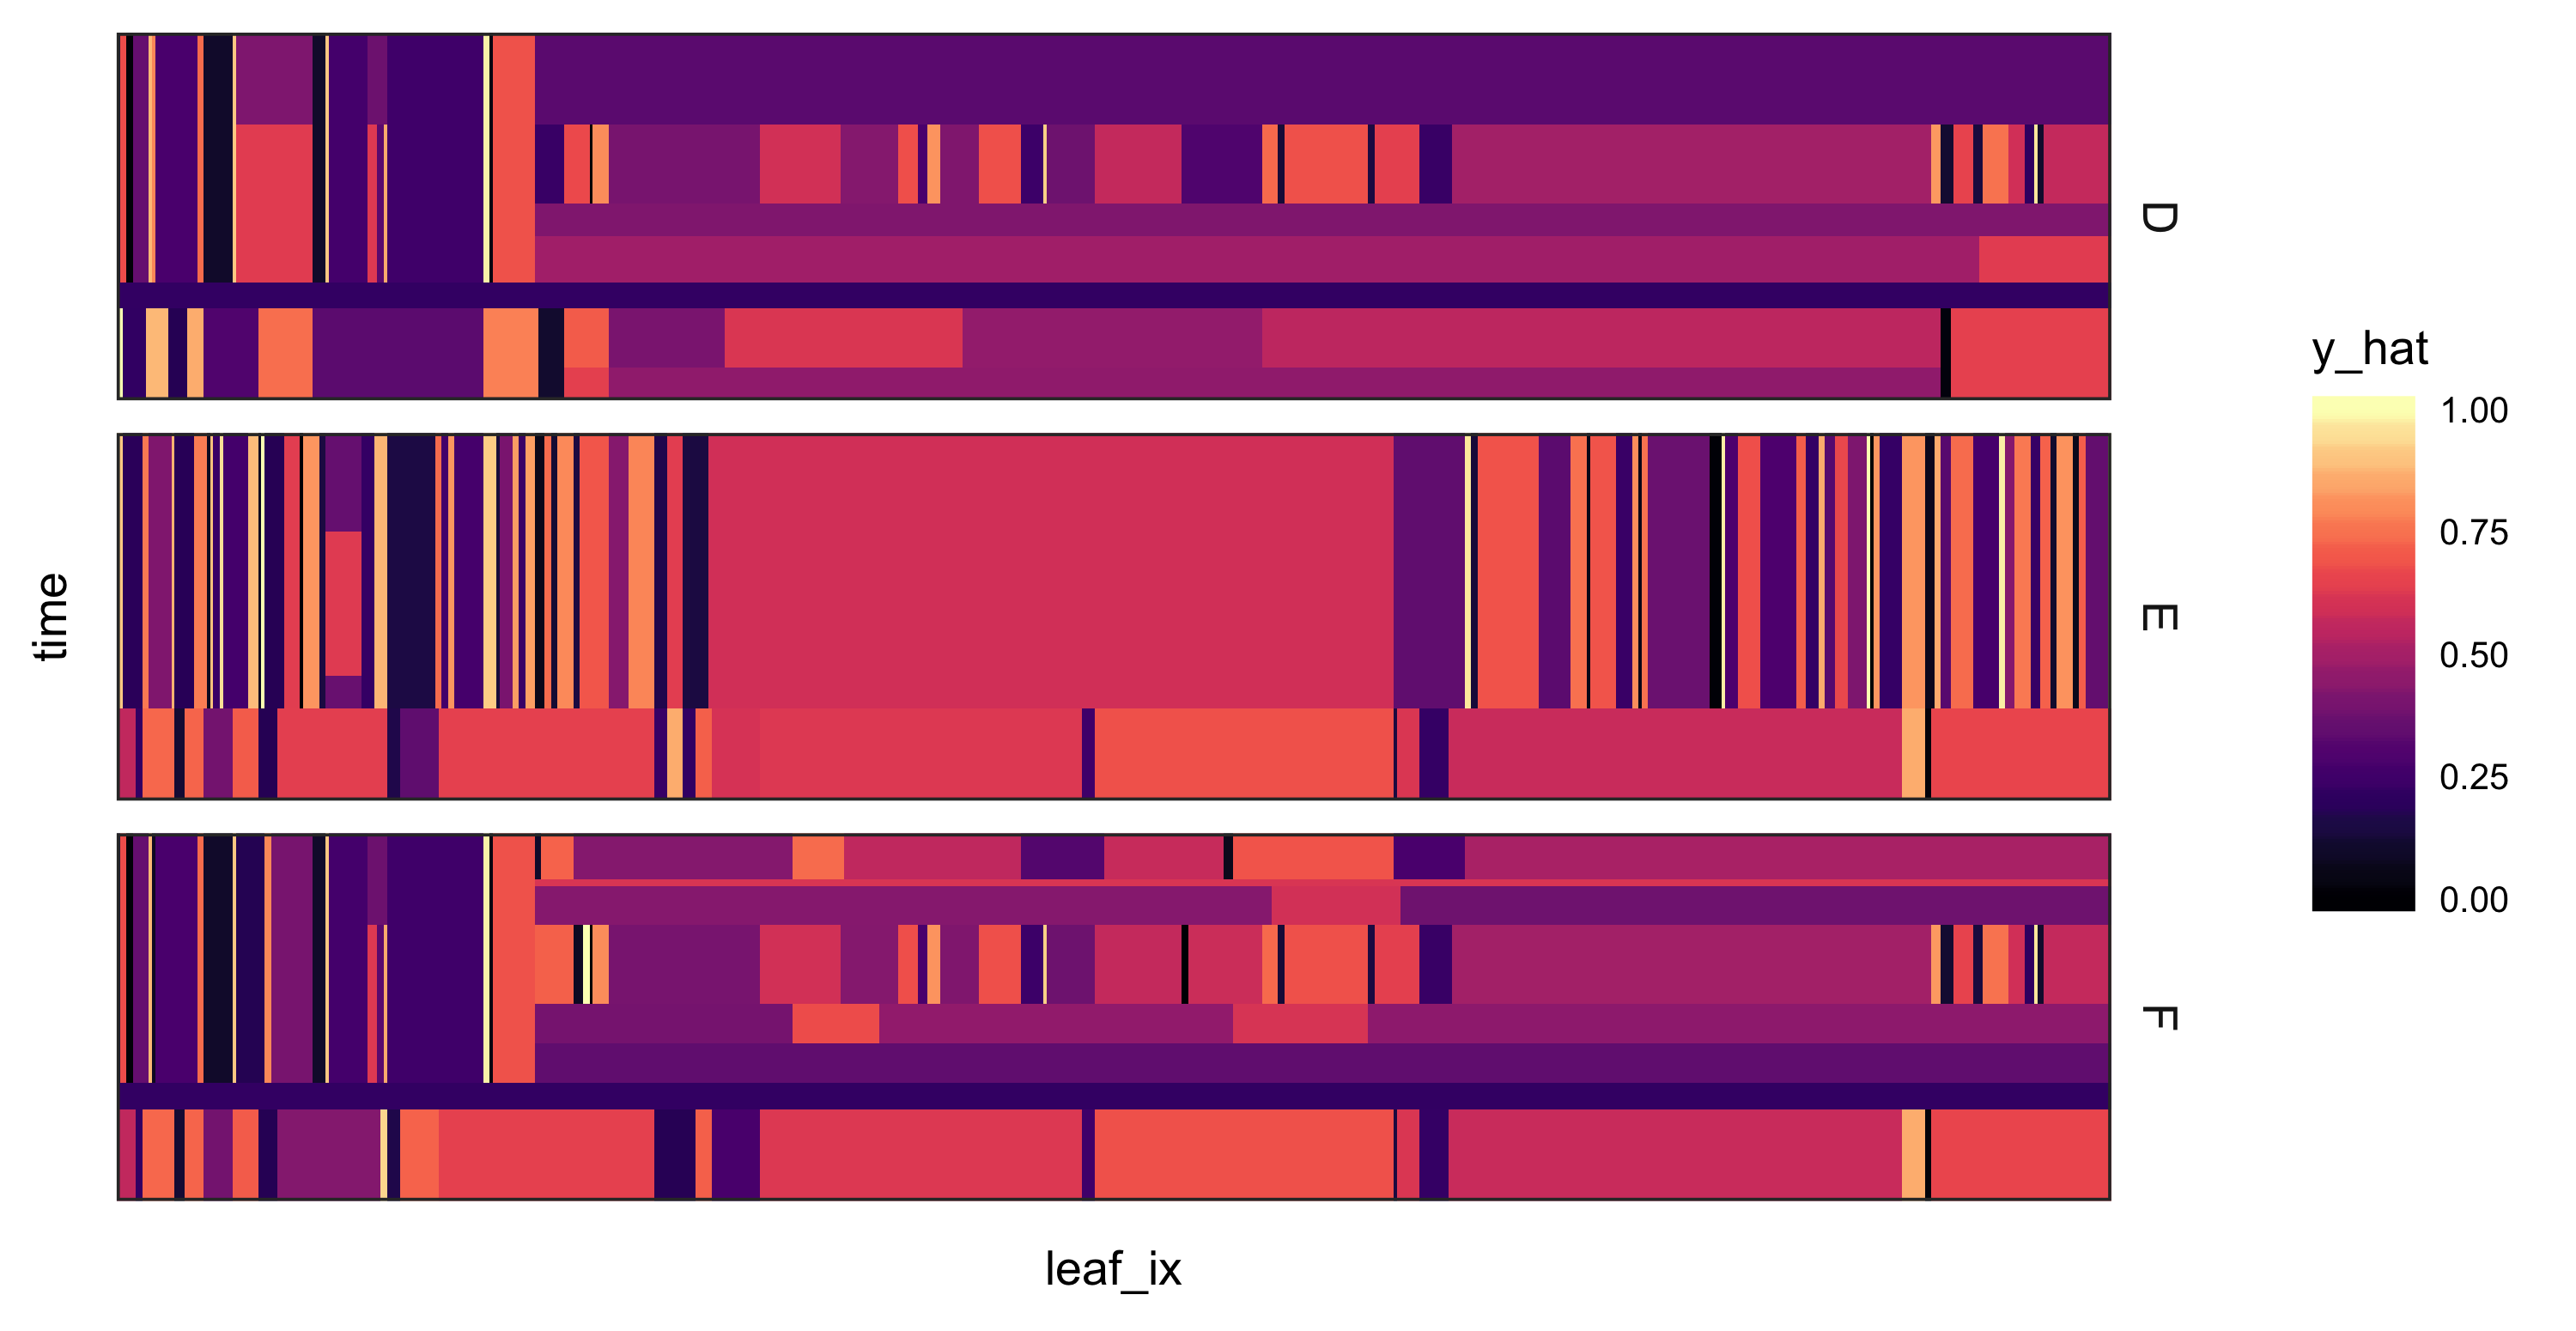
\includegraphics[width=.8\textwidth]{figure/rpart_binary}
    \caption{We can use the same method on presence-absence data, to identify
      whether certain regimes have many more exact zeros than others.
      \label{fig:rpart_binary} }
  \end{figure}
\end{frame}

\begin{frame}
  \frametitle{Sparse Time Series}
\begin{figure}[ht]
  \centering
  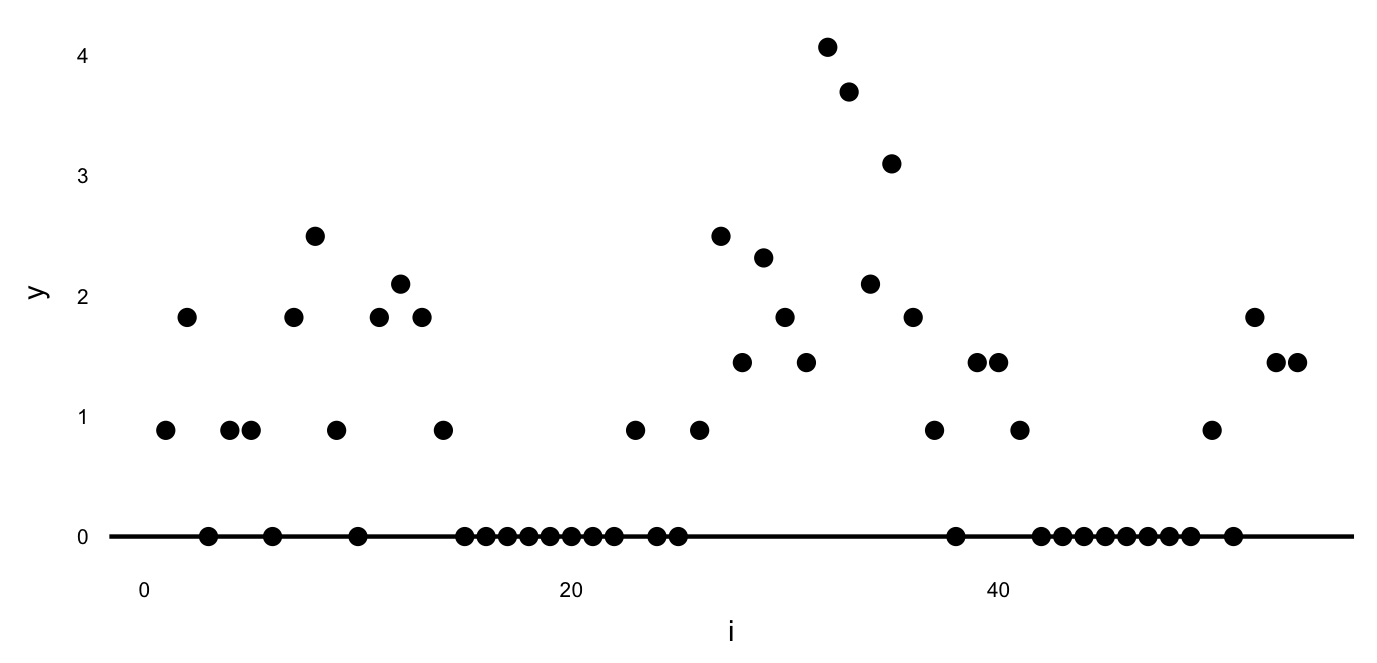
\includegraphics[width=0.9\textwidth]{figure/abt_zeros}
  \caption{One species from the antibiotics data set. It appears to have
    disappeared during the two antibiotics time courses. There is potentially
    value in modeling sequences of exact zeros in some regimes.
    \label{fig:abt_zeros} }
\end{figure}
\end{frame}

\subsection{Dynamic Tobit}
\label{subsec:dynamic_tobit}

\begin{frame}
  \frametitle{Dynamic Tobit Model}
  \begin{itemize}
  \item To model sparsity in microbiome abundances, we can adopt a censoring
    point of view
  \item For example, the Dynamic Tobit model adds an extra layer of censoring on
    top of the ordinary state space model,
    \begin{align*}
      x_{t} &= Ax_{t - 1} + w_{t} \\
      \tilde{y}_{t} &= Cx_{t} + \eps_{t} \\
      y_{t} &= \tilde{y}_{t} \indic{\tilde{y}_{t} \geq c},
    \end{align*}
    where both $x$ and $\tilde{y}$ are unobserved.
  \item MCMC \citep{de1997scan, brockwell2006long, manrique1998simulation} and
    particle filtering \citep{andrieu2002particle} approaches are available
  \item Note this does not share information across species
  \end{itemize}
\end{frame}

\begin{figure}
  \frametitle{Antibiotics Example}
  \centering
  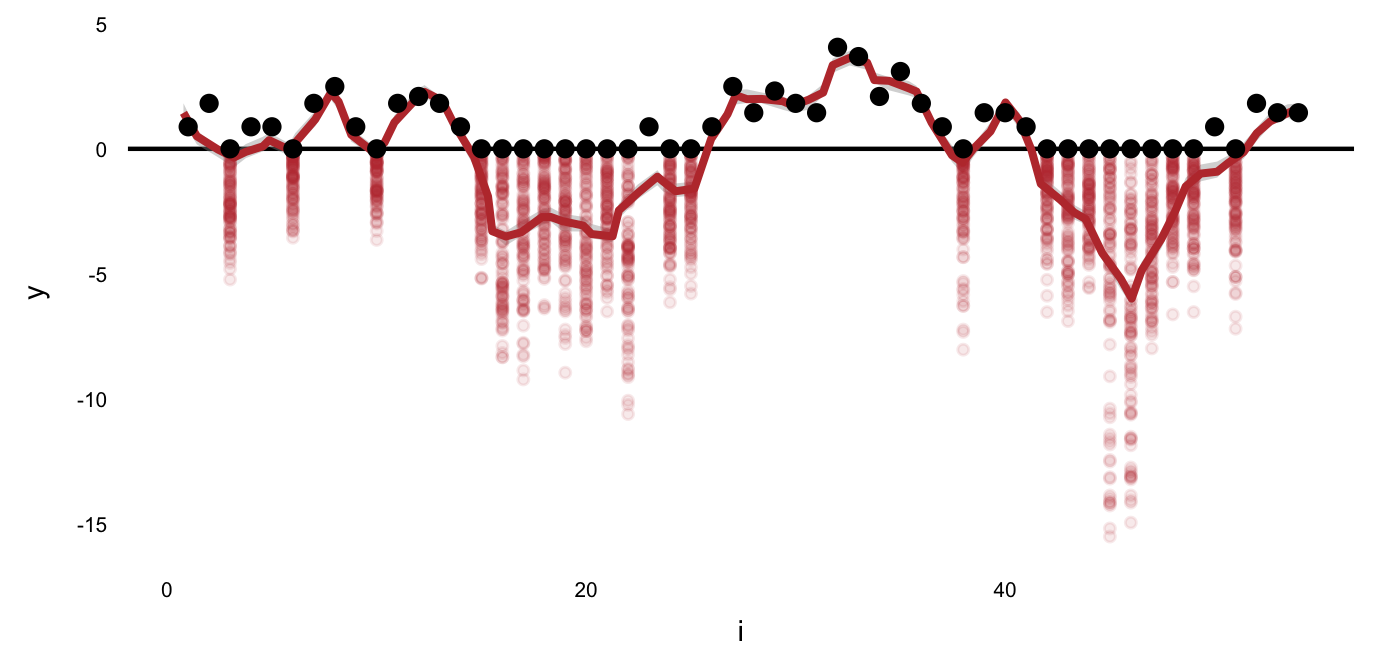
\includegraphics[width=\textwidth]{figure/abt_scan}
  \caption{Results of the scan sampler for a single species. Black points are
    observed data, red points are posterior samples, and the red line is a
    kernel smooth over samples. Implementation at
    \url{https://github.com/krisrs1128/readings/} \label{fig:abt_scan}
  }
\end{figure}

\subsection{Mixture of GPs}
\label{subsec:mix_gps}

\begin{frame}
  \frametitle{Mixture of GPs}
  \begin{itemize}
  \item Gaussian Processes (GPs) provide an alternative to dynamical systems for
    working with functional data
  \item GPs are well-suited to homogeneous data, but cannot model regime
    switching directly, because the kernel bandwidth is constant
  \end{itemize}

  \begin{figure}[ht]
    \centering
    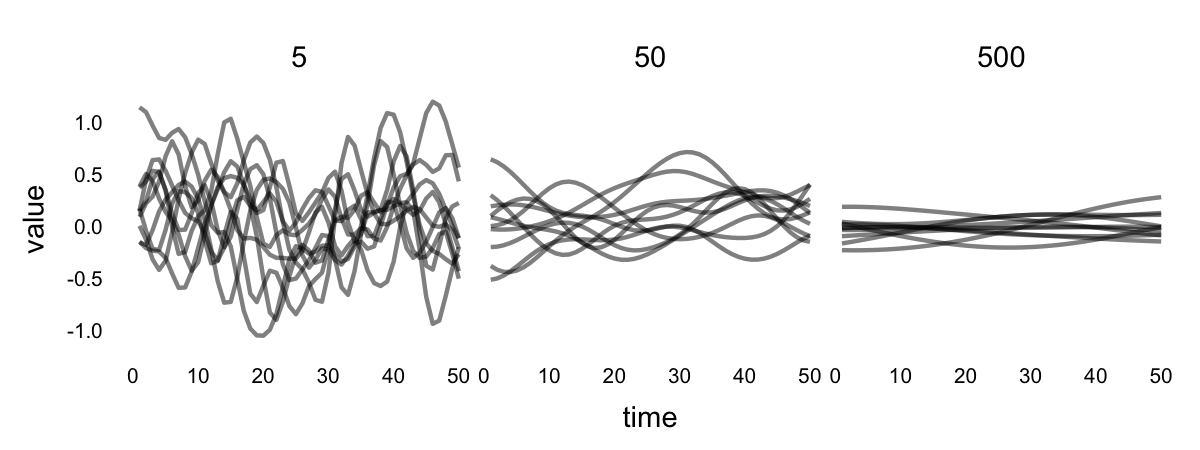
\includegraphics[width=0.8\textwidth]{figure/gp_bandwidths}
    \caption{Different bandwidths in a GP are associated with different dynamics,
      but dynamics cannot switch across timepoints. \label{fig:gp_bandwidths} }
  \end{figure}
\end{frame}

\begin{frame}
  \frametitle{Mixture of GPs}
\begin{itemize}
\item To adapt GPs to more heterogeneous situations, many mixture
  \citep{tresp2001mixtures, rasmussen2002infinite}, multiscale
  \citep{fox2012multiresolution, samostring}, and time-varying
  \citep{paciorek2003nonstationary} approaches have been proposed
\item We focus on the formulation of \citep{rasmussen2002infinite},
 \begin{align*}
   y\left(t_{i}\right) \vert \{ \text{class}\left(t_{i}\right) = k\} &\sim
   \Gsn\left(x_{k}\left(t_{i}\right), \sigma^{2}\right) \\
   x_{k}\left(t\right) &\sim \GP\left(0, \kappa_{k}\right)  \\
   \left[\text{class}\left(t_{i}\right)\right] &\sim \text{CRP}\left(\alpha\right)
 \end{align*}
\end{itemize}
\end{frame}

\begin{frame}
  \frametitle{Aside: Implementation tricks}
  \begin{itemize}
  \item Inference is accomplished by alternating gibbs sampling of class
    assignments with HMC on kernel hyperparameters. Code at
    \url{https://github.com/krisrs1128/readings} (\texttt{igp\_mix} folder).
  \item Can check gibbs sampling conditionals by evaluating $\frac{p\left(x
    \vert z\right)}{p\left(x^{\prime} \vert z\right)} = \frac{p\left(x,
      z\right)}{p\left(x^{\prime}, z\right)}$ at two random points, since
    complete data likelihood is much easier to evaluate than conditional
    \citep{grosse2014testing}
  \item Can check HMC derivatives using numerical derivative calculations
  \item Can use generic HMC packages, plugging in problem specific densities /
    gradients
  \end{itemize}
\end{frame}

\begin{frame}
  \frametitle{Antibiotics Data}
\begin{figure}[ht]
  \centering
  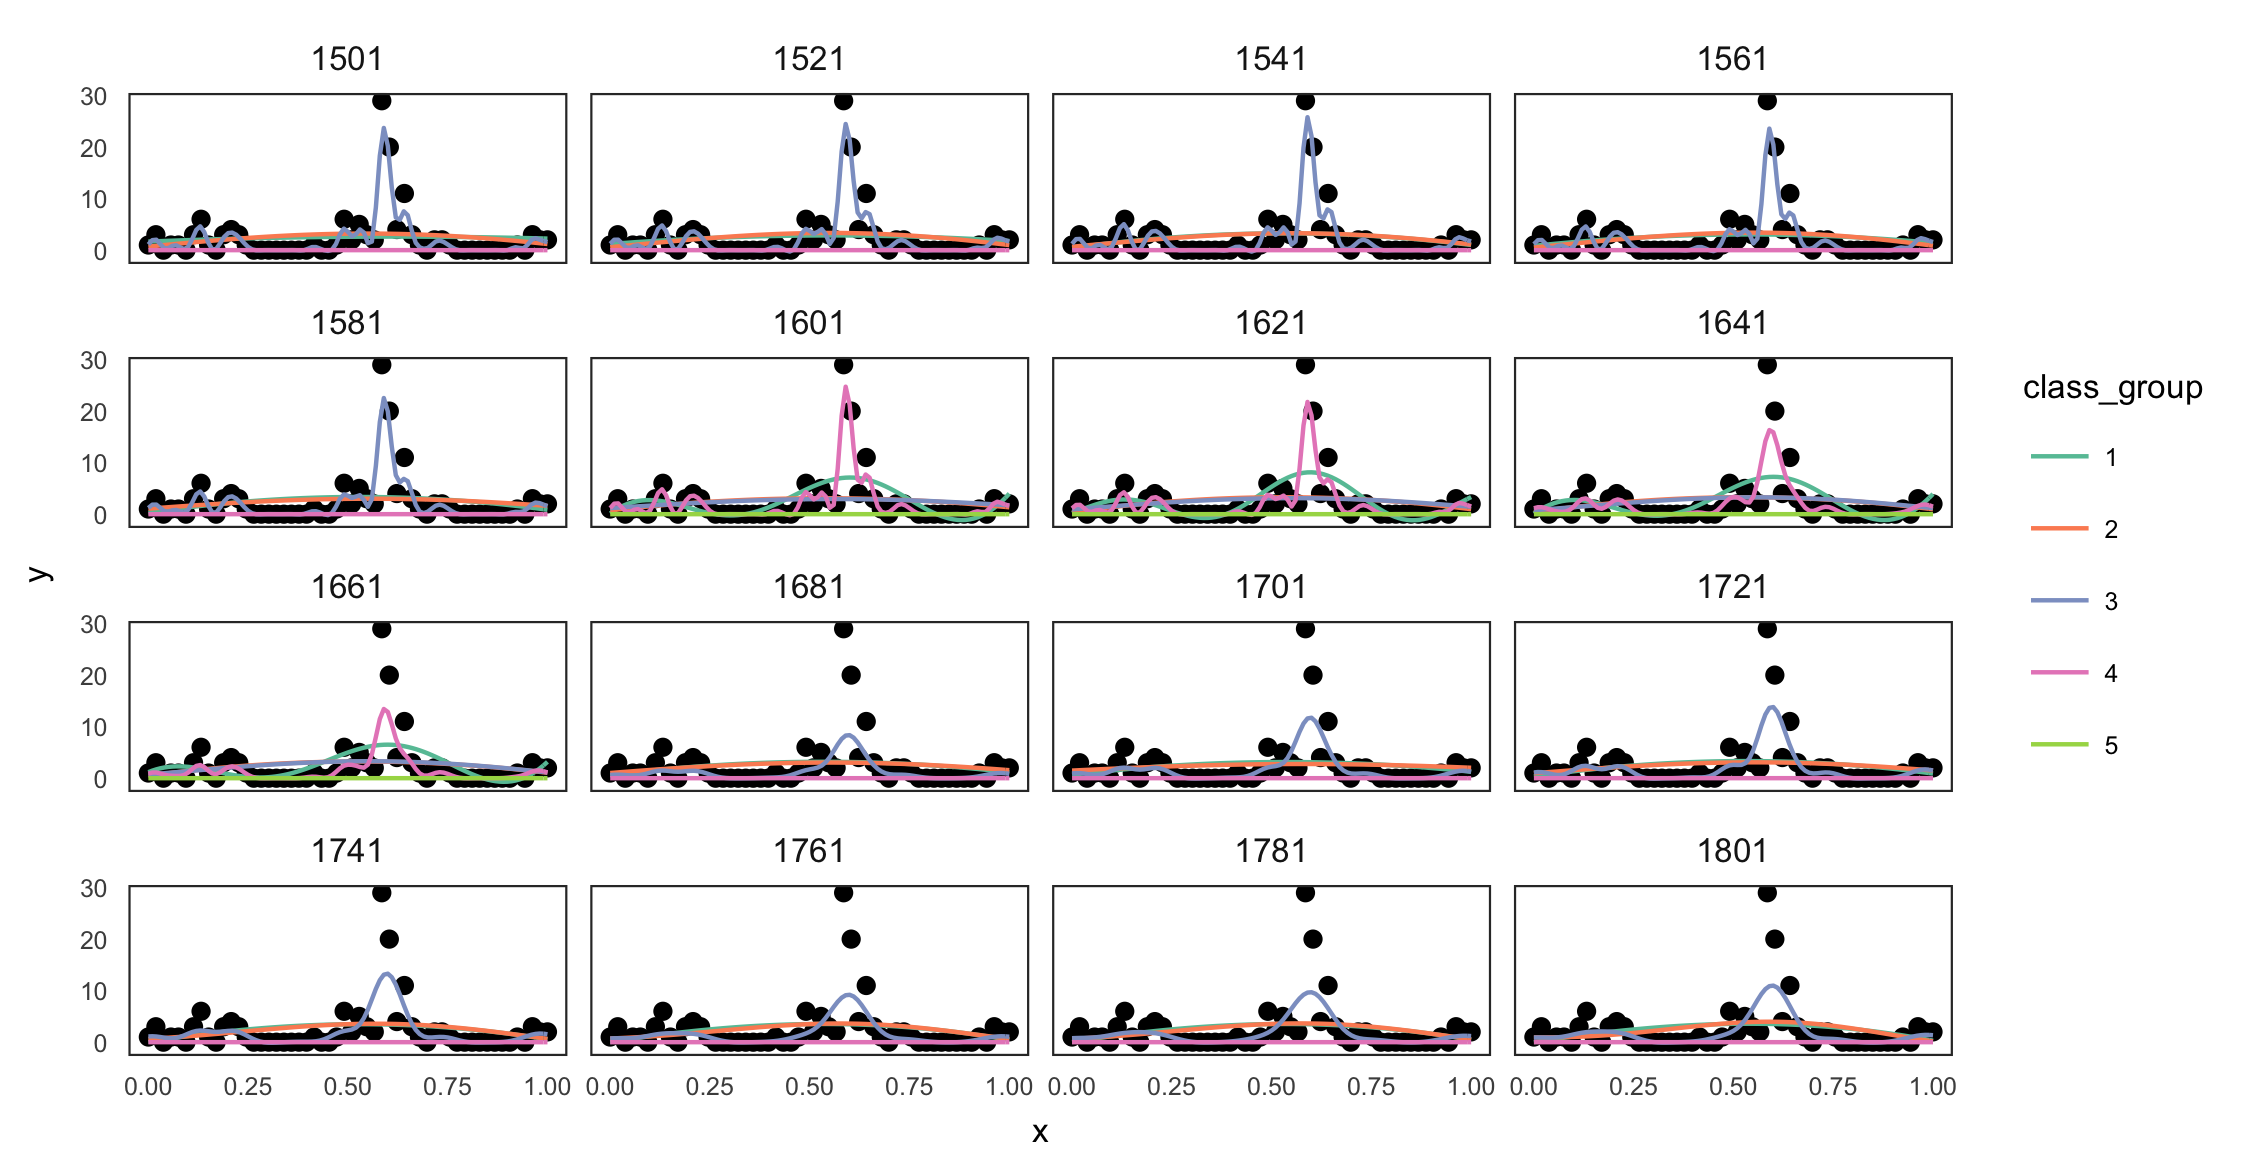
\includegraphics[width=0.8\textwidth]{figure/abt_fits}
  \caption{Each panel represents displays the posteriors at one
    iteration of the sampler. Posteriors for each process are displayed over the
    full data range, even when the associated timepoints occupy a relatively
    restricted range. \label{fig:abt_fits}}
\end{figure}
\end{frame}

\begin{frame}
  \frametitle{Antibiotics Data}
\begin{figure}[ht]
  \centering
  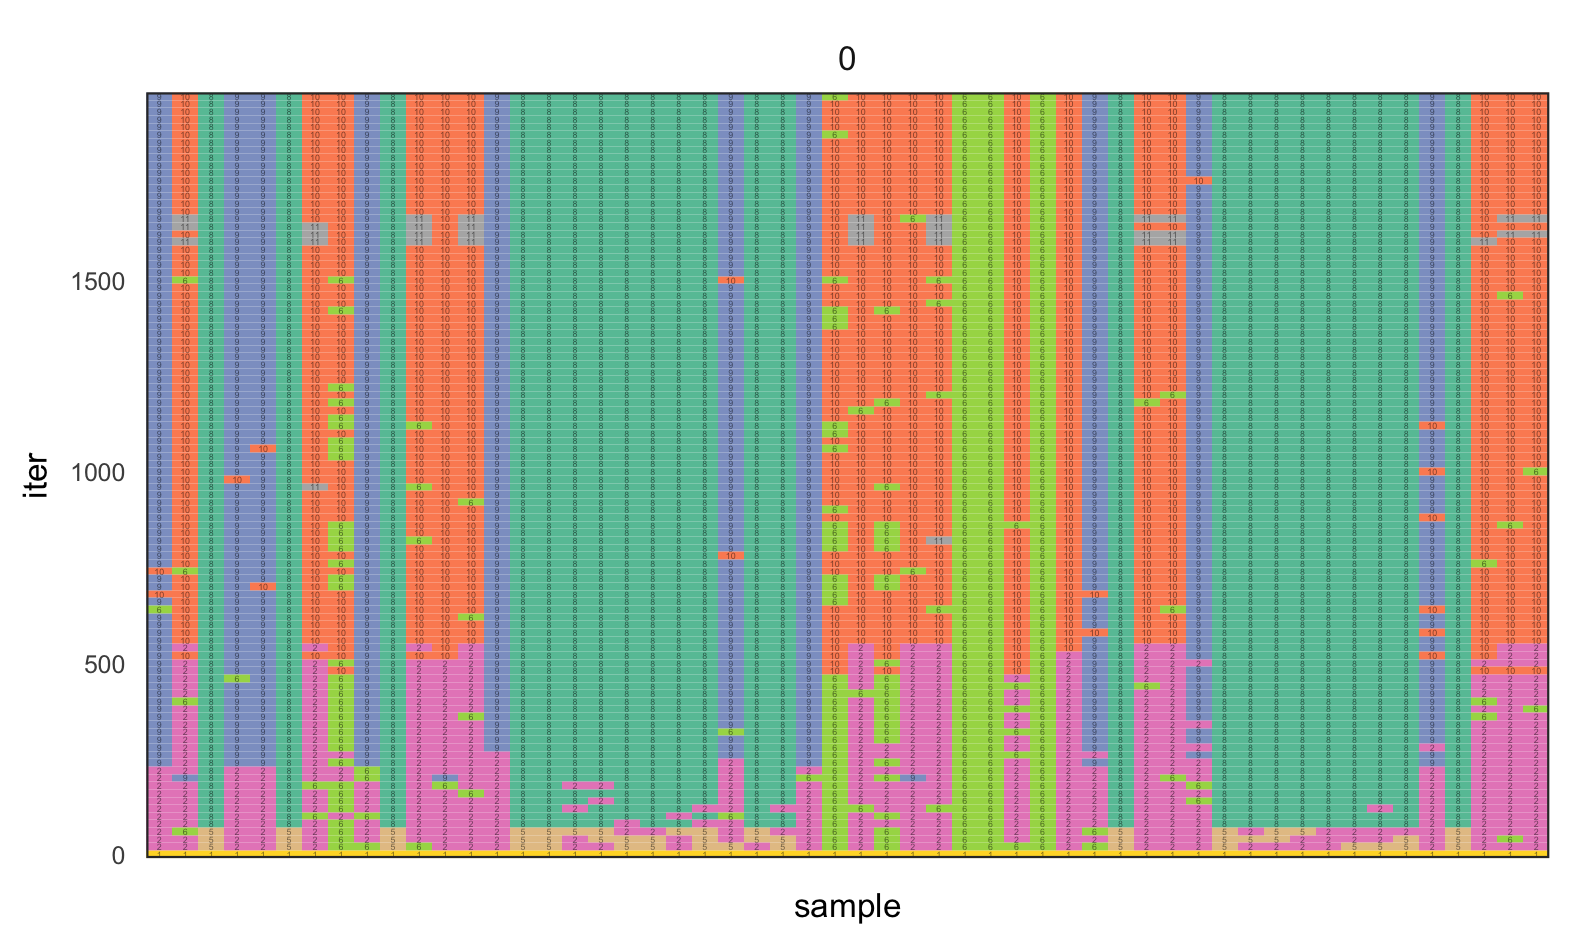
\includegraphics[width=0.7\textwidth]{figure/abt_states}
  \caption{Each row is an iteration of the sampler, each column is a timepoint.
    Tiles are shaded by their class assignments. Note the label switching that
    occurs a few times. \label{fig:abt_states} }
\end{figure}
\end{frame}

\begin{frame}
  \frametitle{Antibiotics Data}
\begin{figure}[ht]
  \centering
  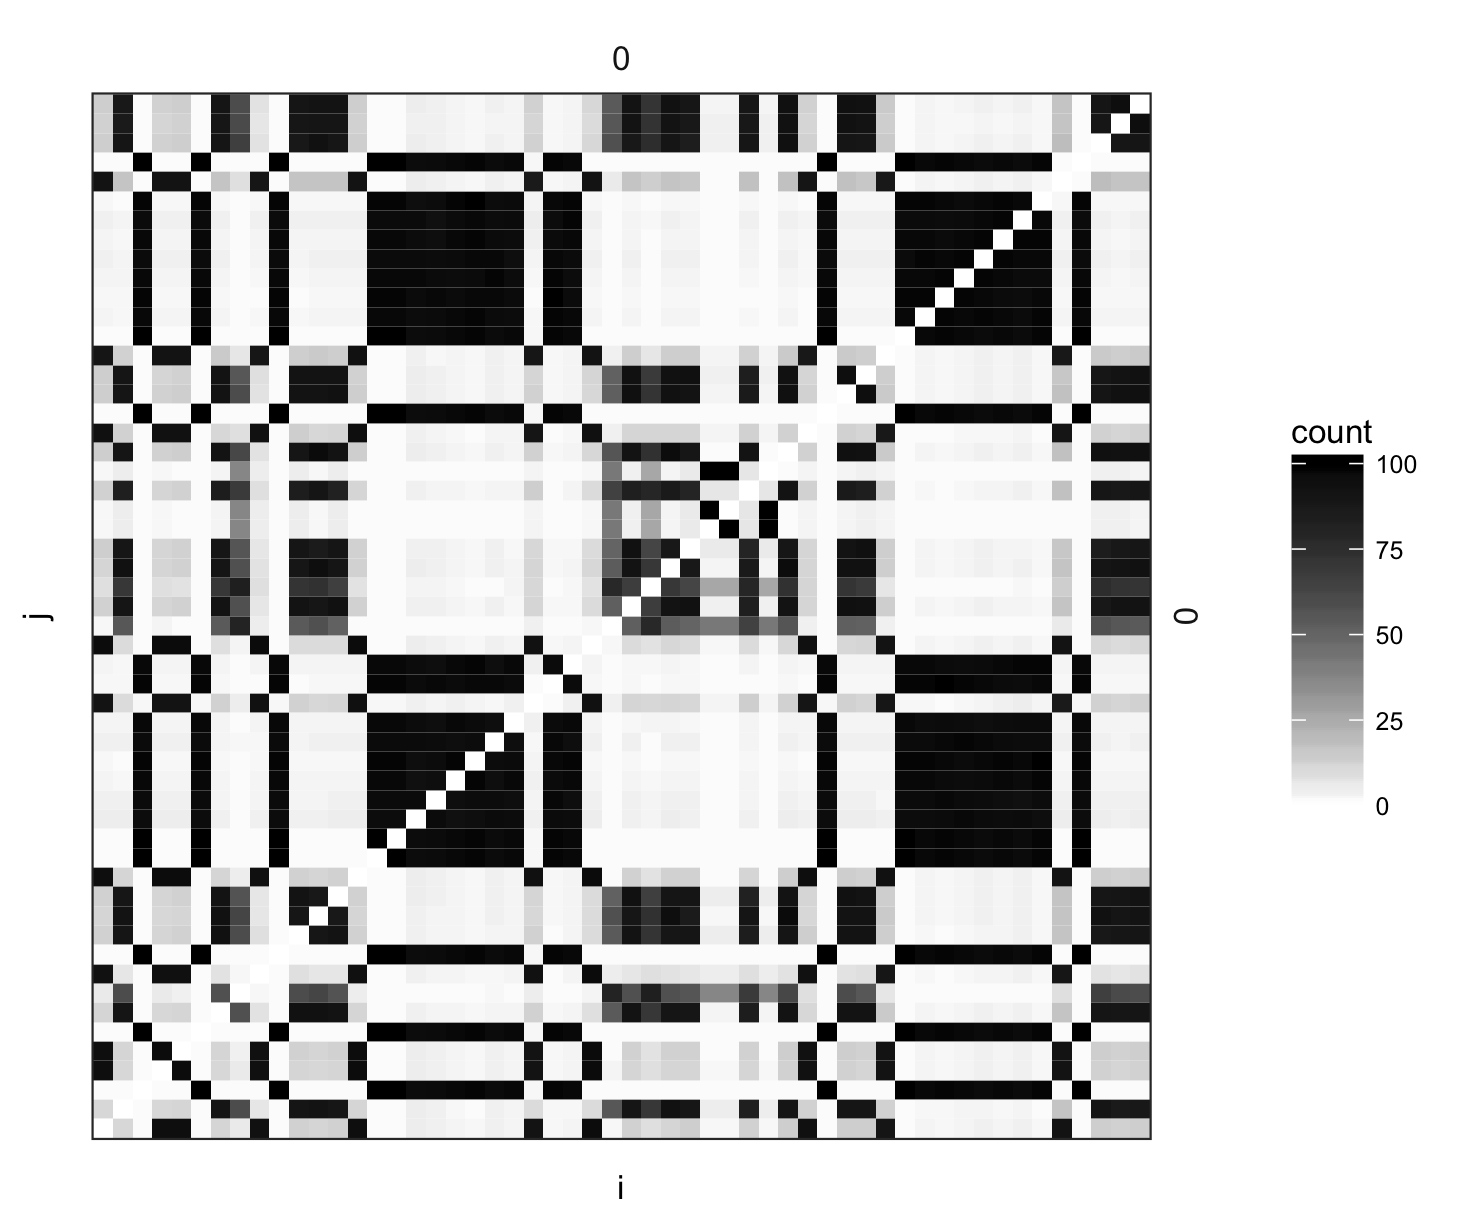
\includegraphics[width=0.5\textwidth]{figure/abt_cooccurrence}
  \caption{To bypass the label switching problem, we can count how often two
    timepoints were placed in the same cluster (this statistic is invariant to
    switching). We see clear antibiotic regime groups. \label{afig:abt_states}}
\end{figure}
\end{frame}

\subsection{Changepoint detection}
\label{subsec:changpoint}

\begin{frame}
  \frametitle{Changepoint Detection}
  \begin{itemize}
  \item While there are many proposals for changepoint detection within
    individual series, few methods leverage information across multiple series
  \item \citep{fan2015empirical} proposes an approach (BASIC) for the
    multiple-series situation
  \item They have two insights that lead to statistical and computational
    performance improvements,
    \begin{itemize}
    \item Collapse: Perform sampling directly on cluster assignemnts
    \item Optimize: Can use a numerical Empirical Bayes procedure to avoid
      difficult prior elicitation
    \end{itemize}
  \end{itemize}
\end{frame}

\begin{frame}
  \frametitle{Changepoint Detection}
\begin{figure}[ht]
  \centering
  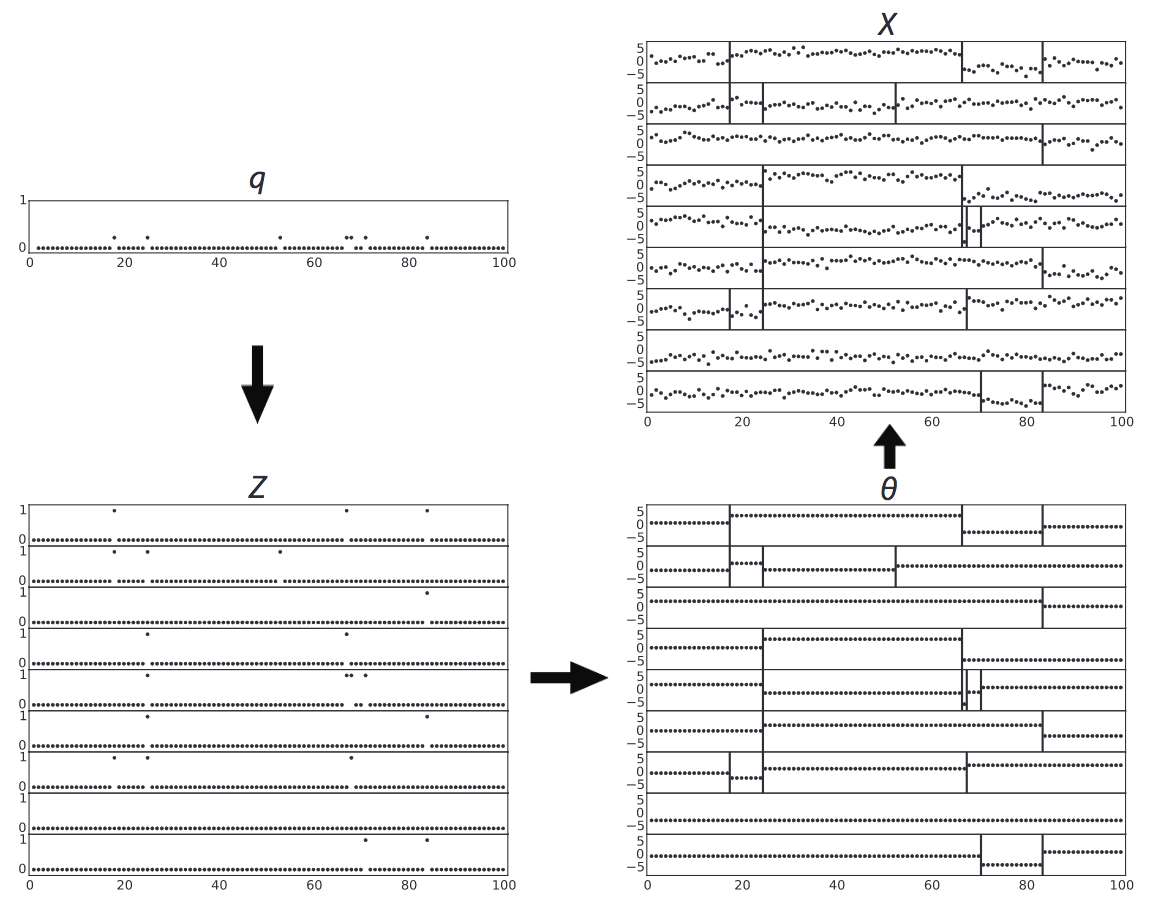
\includegraphics[width=0.6\textwidth]{figure/basic_model}
  \caption{Figure 2 from \citep{fan2015empirical}, illustrating the assumed data
    generating process. \label{fig:basic_model} }
\end{figure}
\end{frame}

\begin{frame}
  \frametitle{Changepoint Detection}
  \begin{itemize}
  \item Model changepoint probabilities $q_{t} \sim \pi_{Q}$, but optimize $\pi_{Q}$ over a class
    \begin{align*}
      \pi_{Q} &= \sum w_{k} \nu_{k}
    \end{align*}
    where $\nu_{k}$ are a prespecified dictionary of densities over $\left[0,
      1\right]$.
  \item Alternately gibbs sample rows and columns, and perform (MCMC-corrected)
    swaps to improve mixing
  \end{itemize}
\end{frame}

\begin{frame}
  \frametitle{Antibiotics Data}
 \begin{figure}[ht]
   \centering
   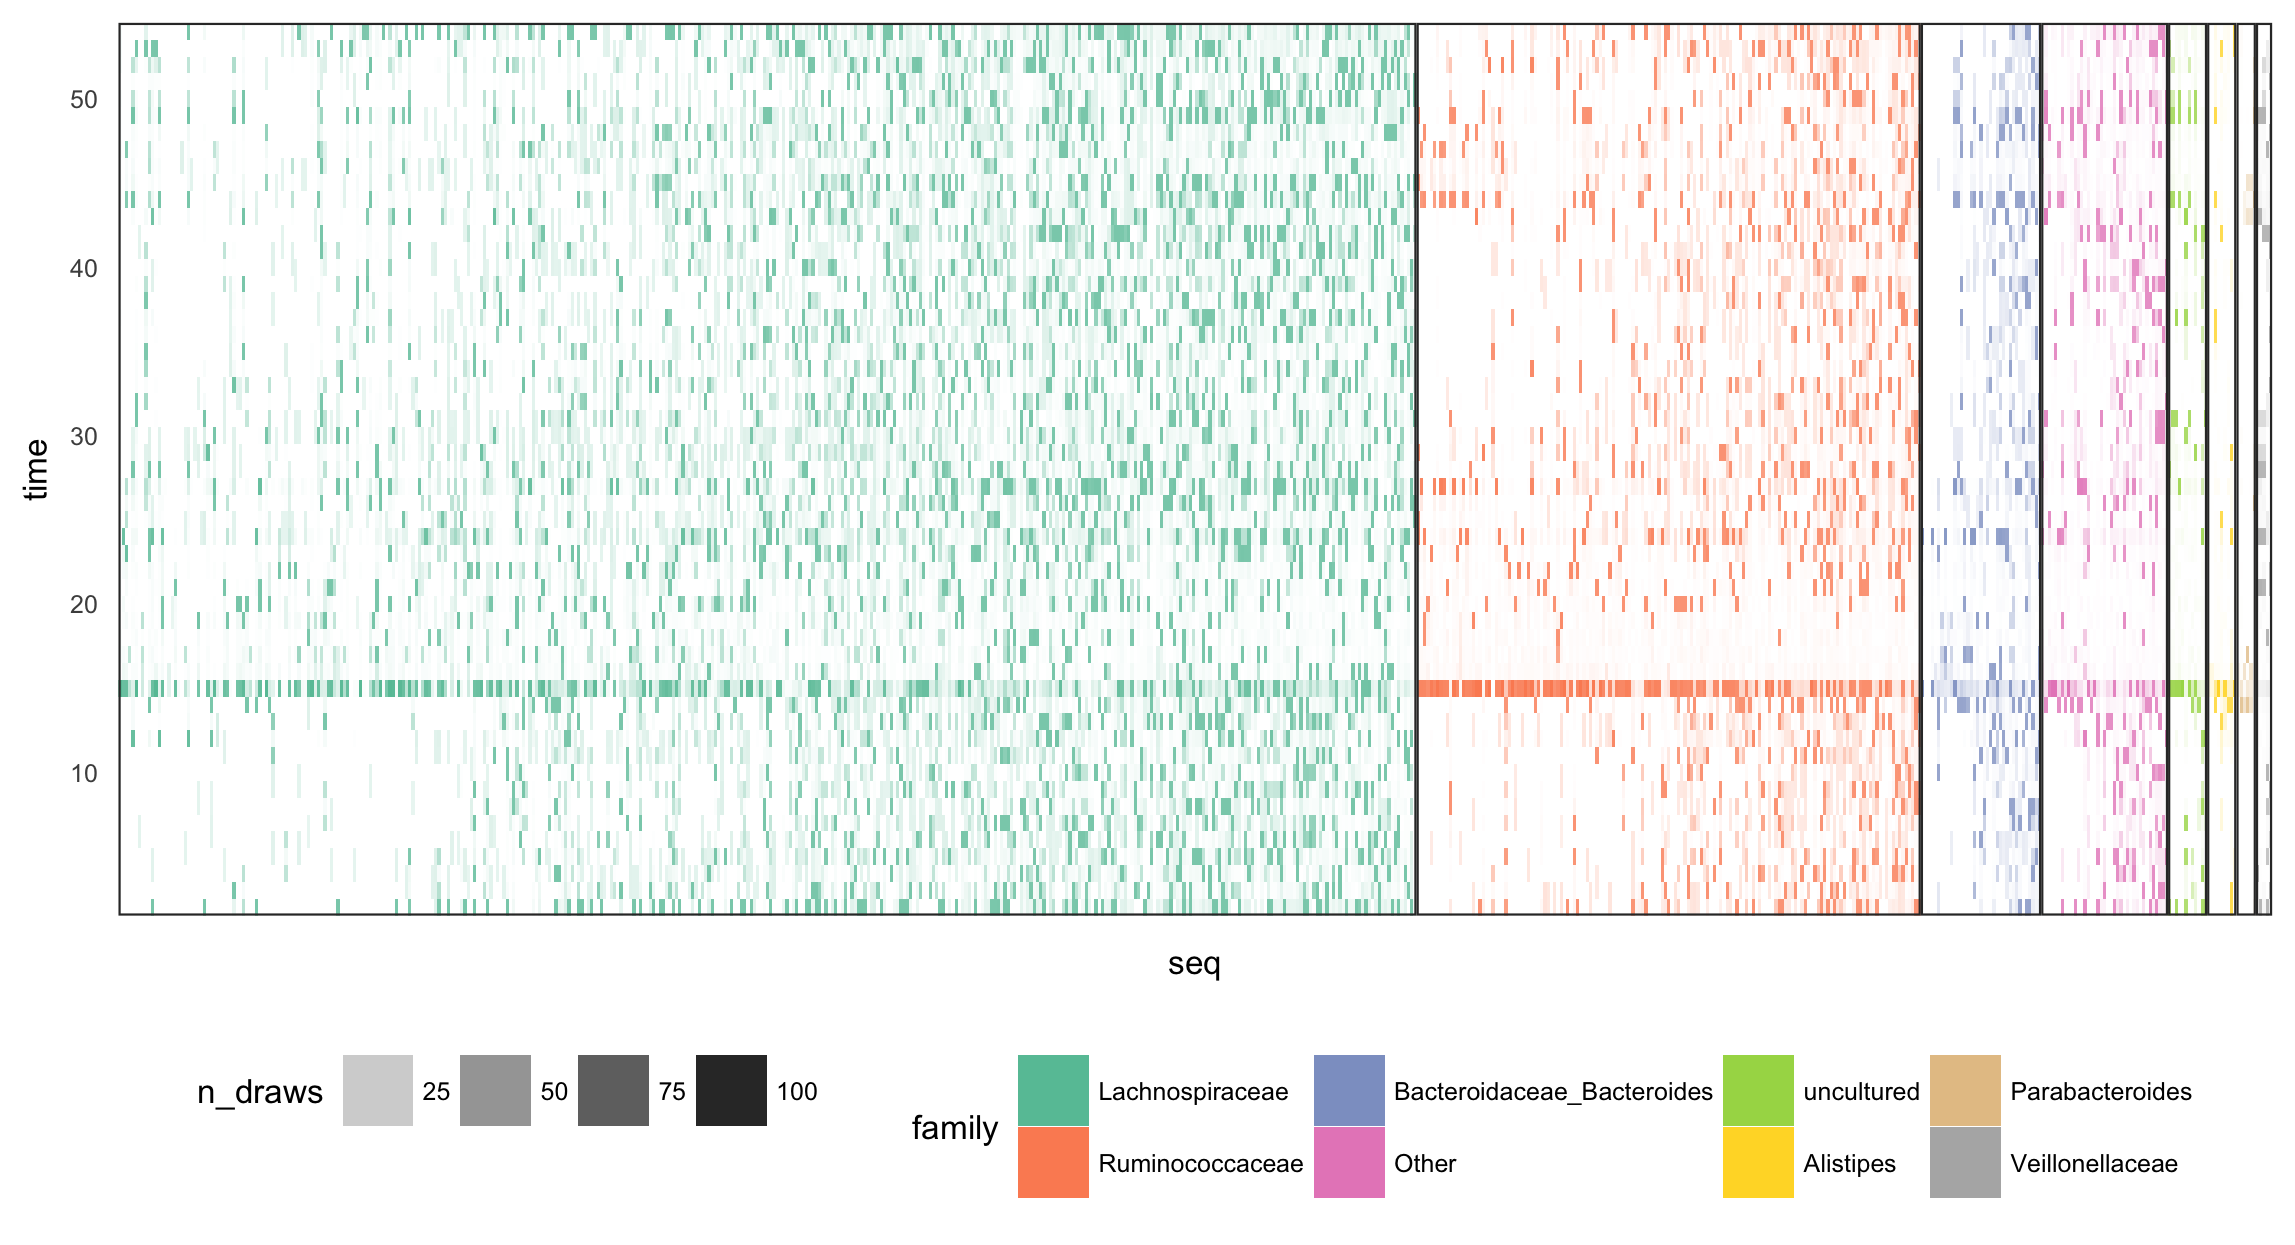
\includegraphics[width=0.8\textwidth]{figure/basic_heatmap}
   \caption{Each column is a species, shaded by its taxonomic family, rows are
     timepoints, and cells are shaded by their posterior changepoint probability
     $p\left(Z_{ij} = 1 \vert X\right)$. \label{fig:basic_heatmap} }
 \end{figure}
\end{frame}

\begin{frame}
  \frametitle{Antibiotics Data}
 \begin{figure}[ht]
   \centering
   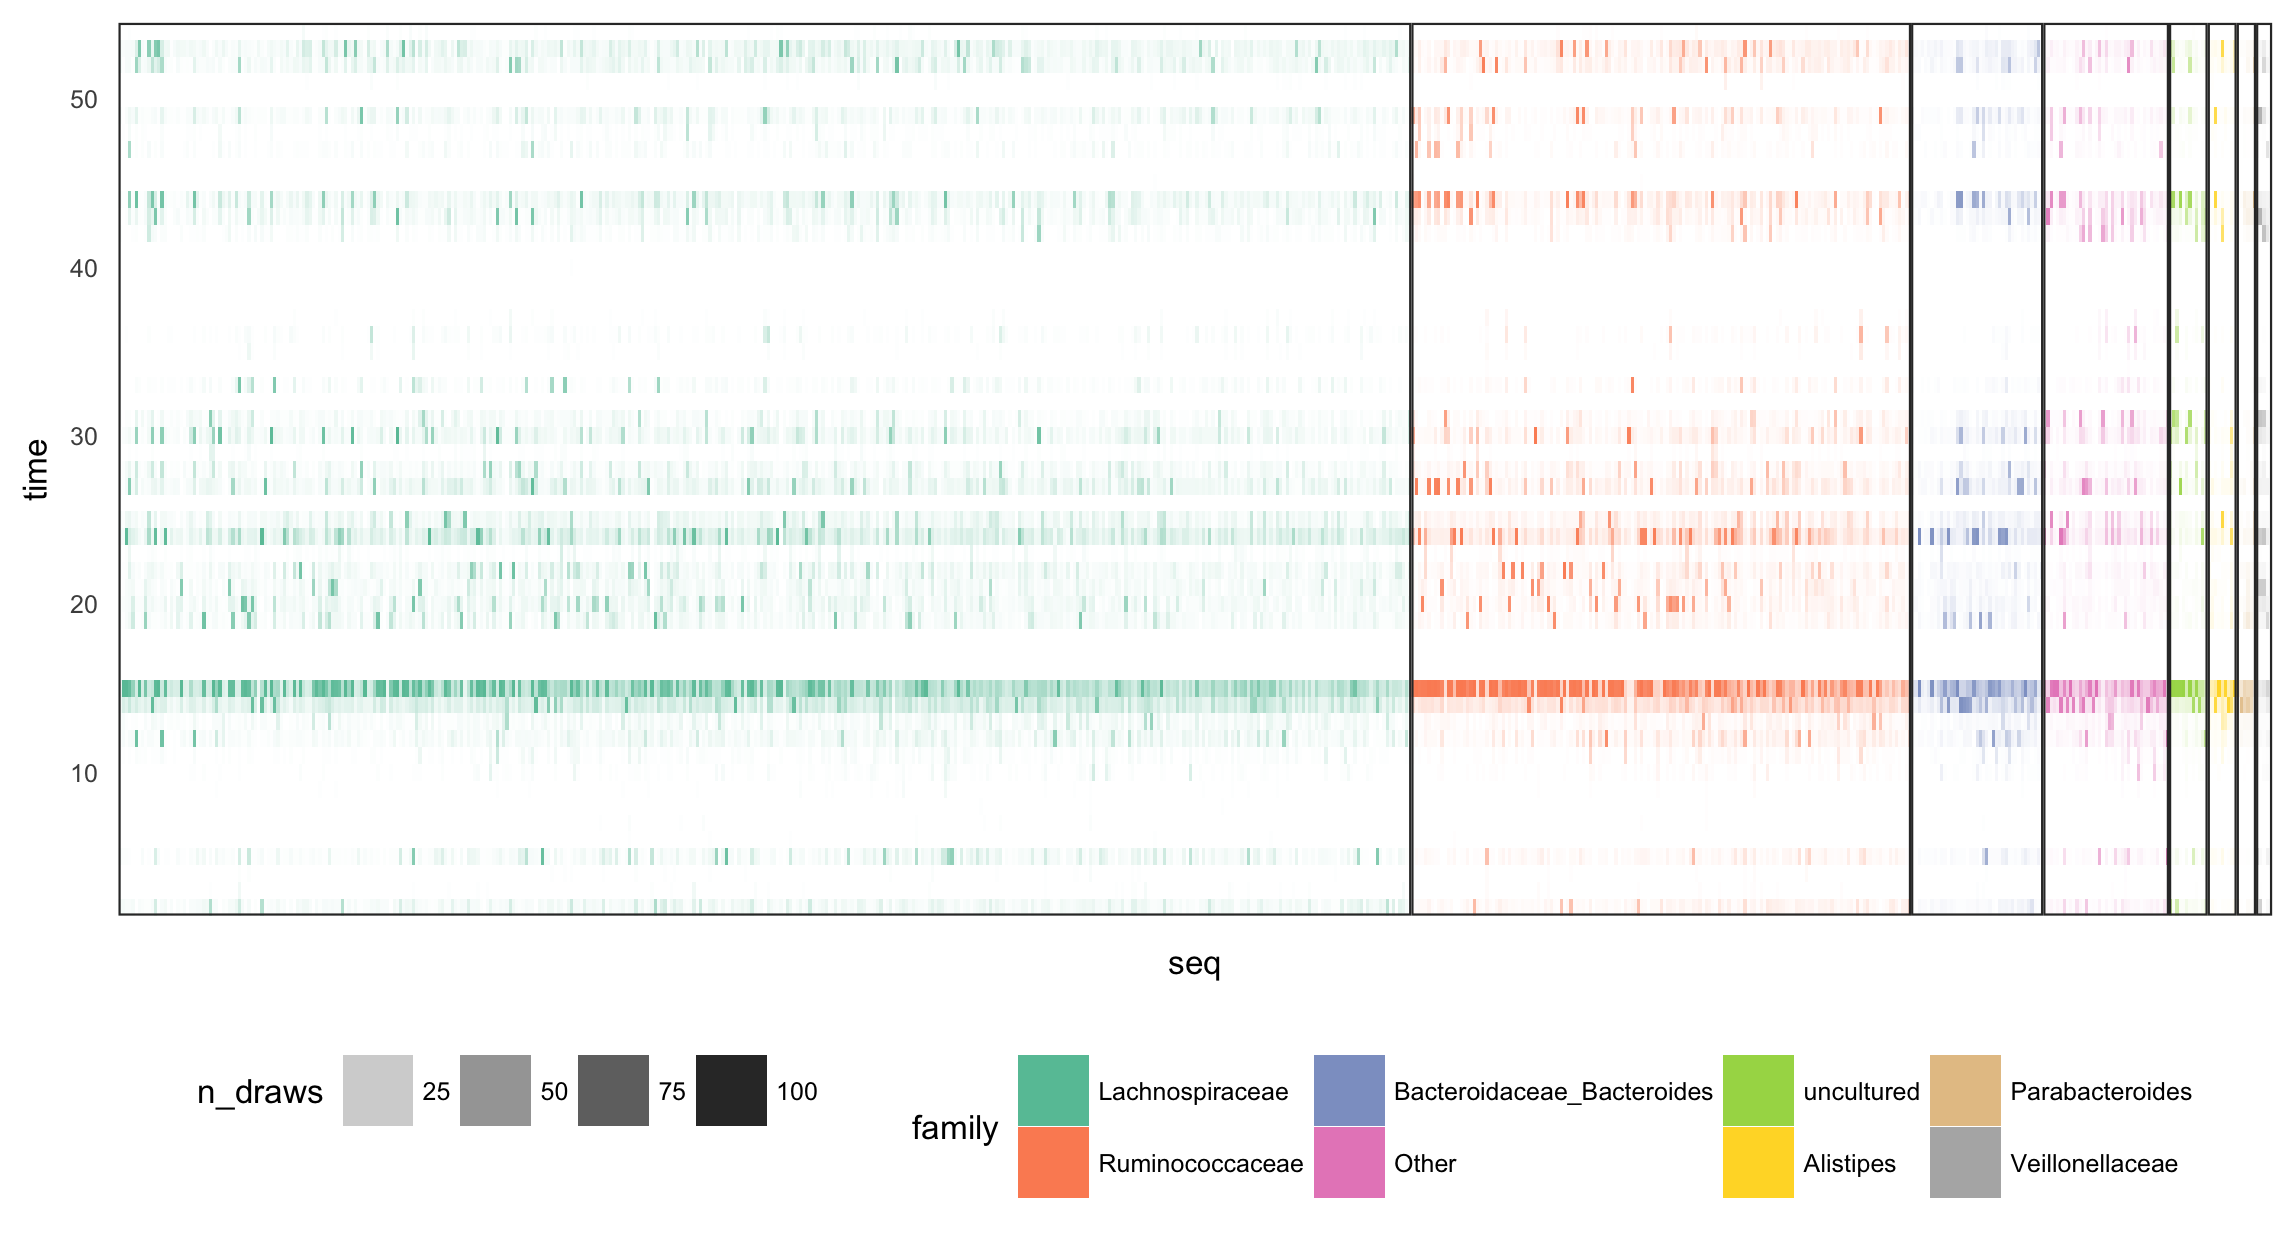
\includegraphics[width=0.8\textwidth]{figure/basic_bern_heatmap}
   \caption{This is the analog of Figure \ref{fig:basic_heatmap}, but with a
     Bernoulli likelihood on the presence / absence data.
     \label{fig:basic_bern_heatmap} }
 \end{figure}
\end{frame}

\section{Multitable Analysis}
\label{sec:multitable analysis}

\begin{frame}
  \frametitle{WELL-China Study}
  \begin{itemize}
  \item Focused on the relationship between various indicators of wellness.
  \item Data about exercise, sleep, diet, mental health for 1969 people, in
    addition to 16s data on 221 participants (with plans for metabolomics,
    methylation, ...)
  \item We focus on the relationship between body composition (lean and fat
    mass) and microbiome structure
  \end{itemize}
\end{frame}

\begin{frame}
  \frametitle{Body Composition}
  \begin{itemize}
  \item Can we reproduce findings relating microbiome and BMI / metabolic
    syndrome, but using richer DXA data on body type?
  \item People with similar BMI might have different disease dispositions
    depending on the distribution of lean and fat mass
  \end{itemize}
\begin{figure}[ht]
  \centering
  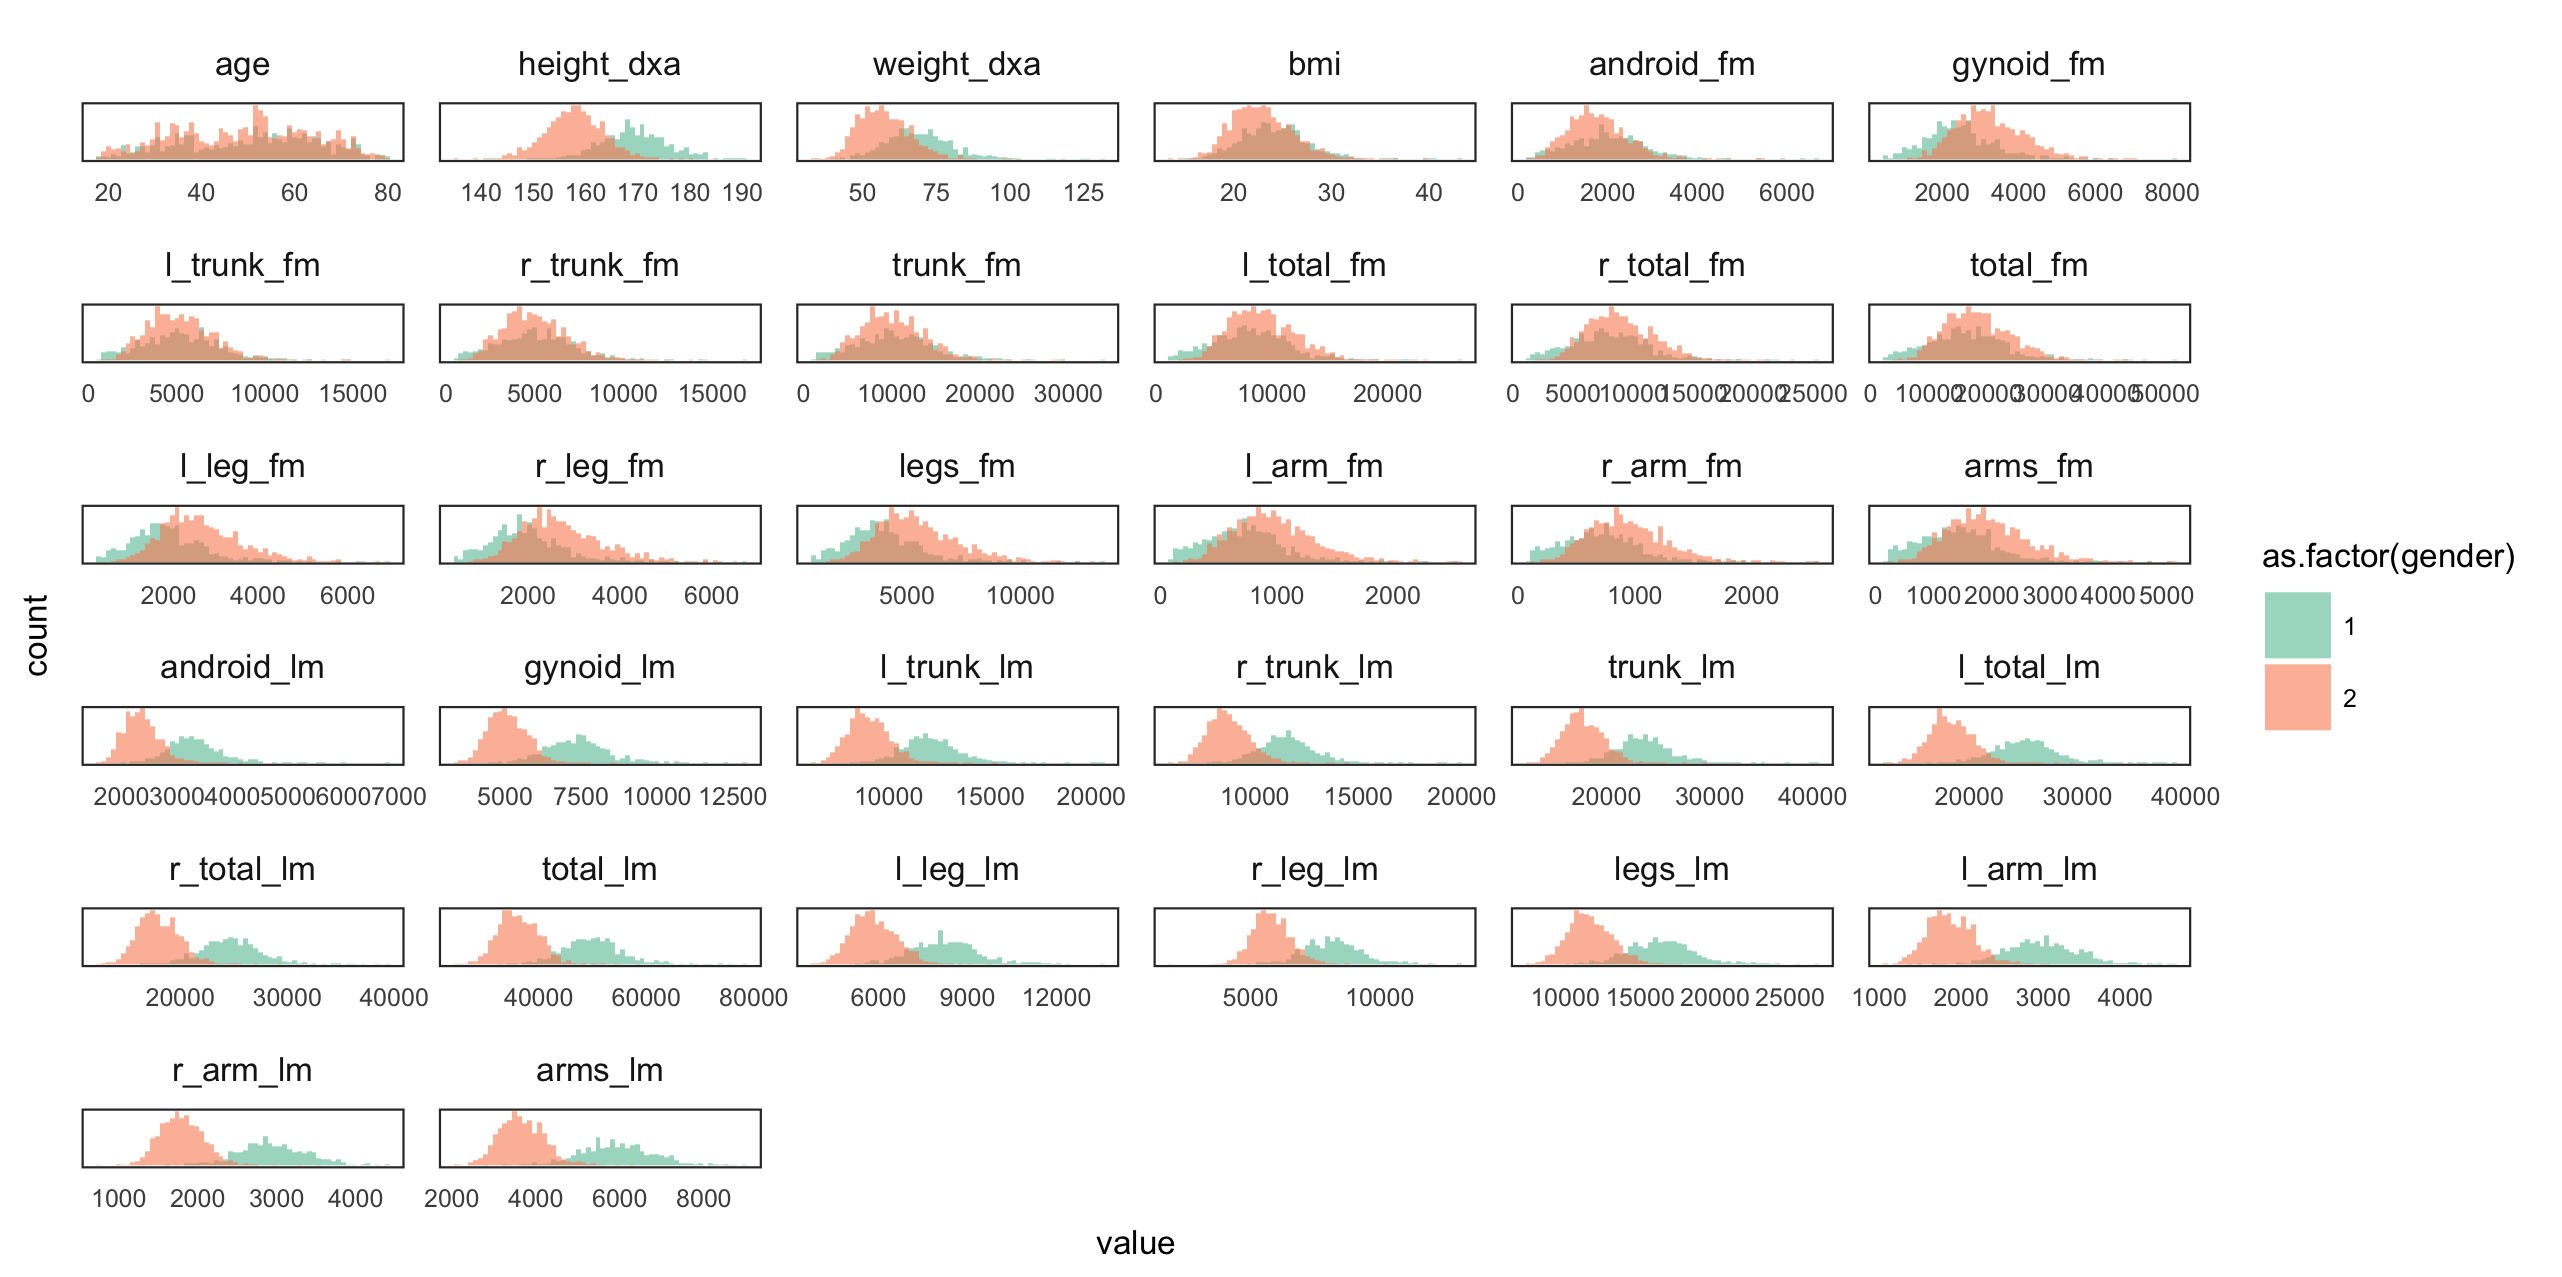
\includegraphics[width=0.65\textwidth]{figure/bc_histo}
  \caption{Marginal distributions of DXA data. \label{fig:bc_histo} }
\end{figure}
\end{frame}
\subsection{PCA}
\label{subsec:pca}

\begin{frame}
  \frametitle{Principal Components Analysis (PCA)}
  \begin{figure}[ht]
    \centering
    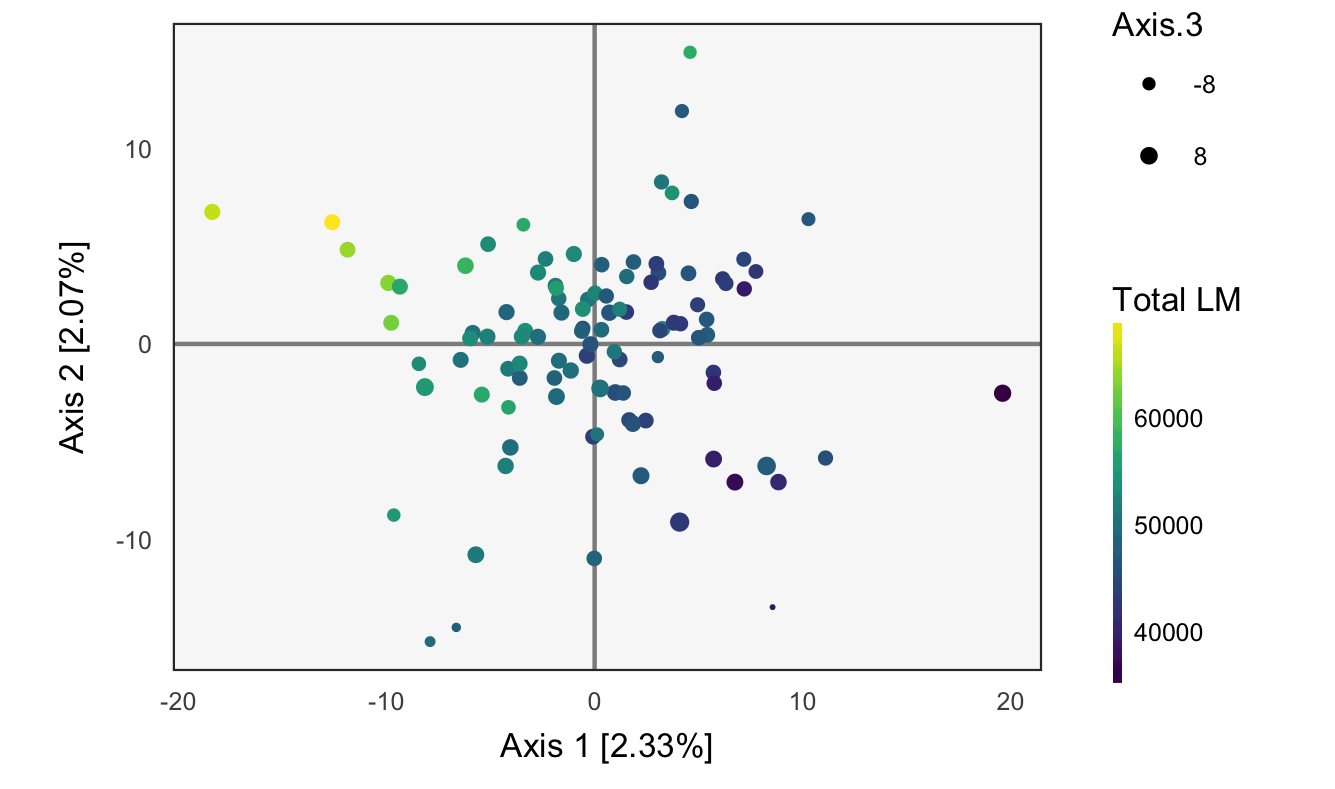
\includegraphics[width=0.45\textwidth]{figure/pca_scores_lm}
    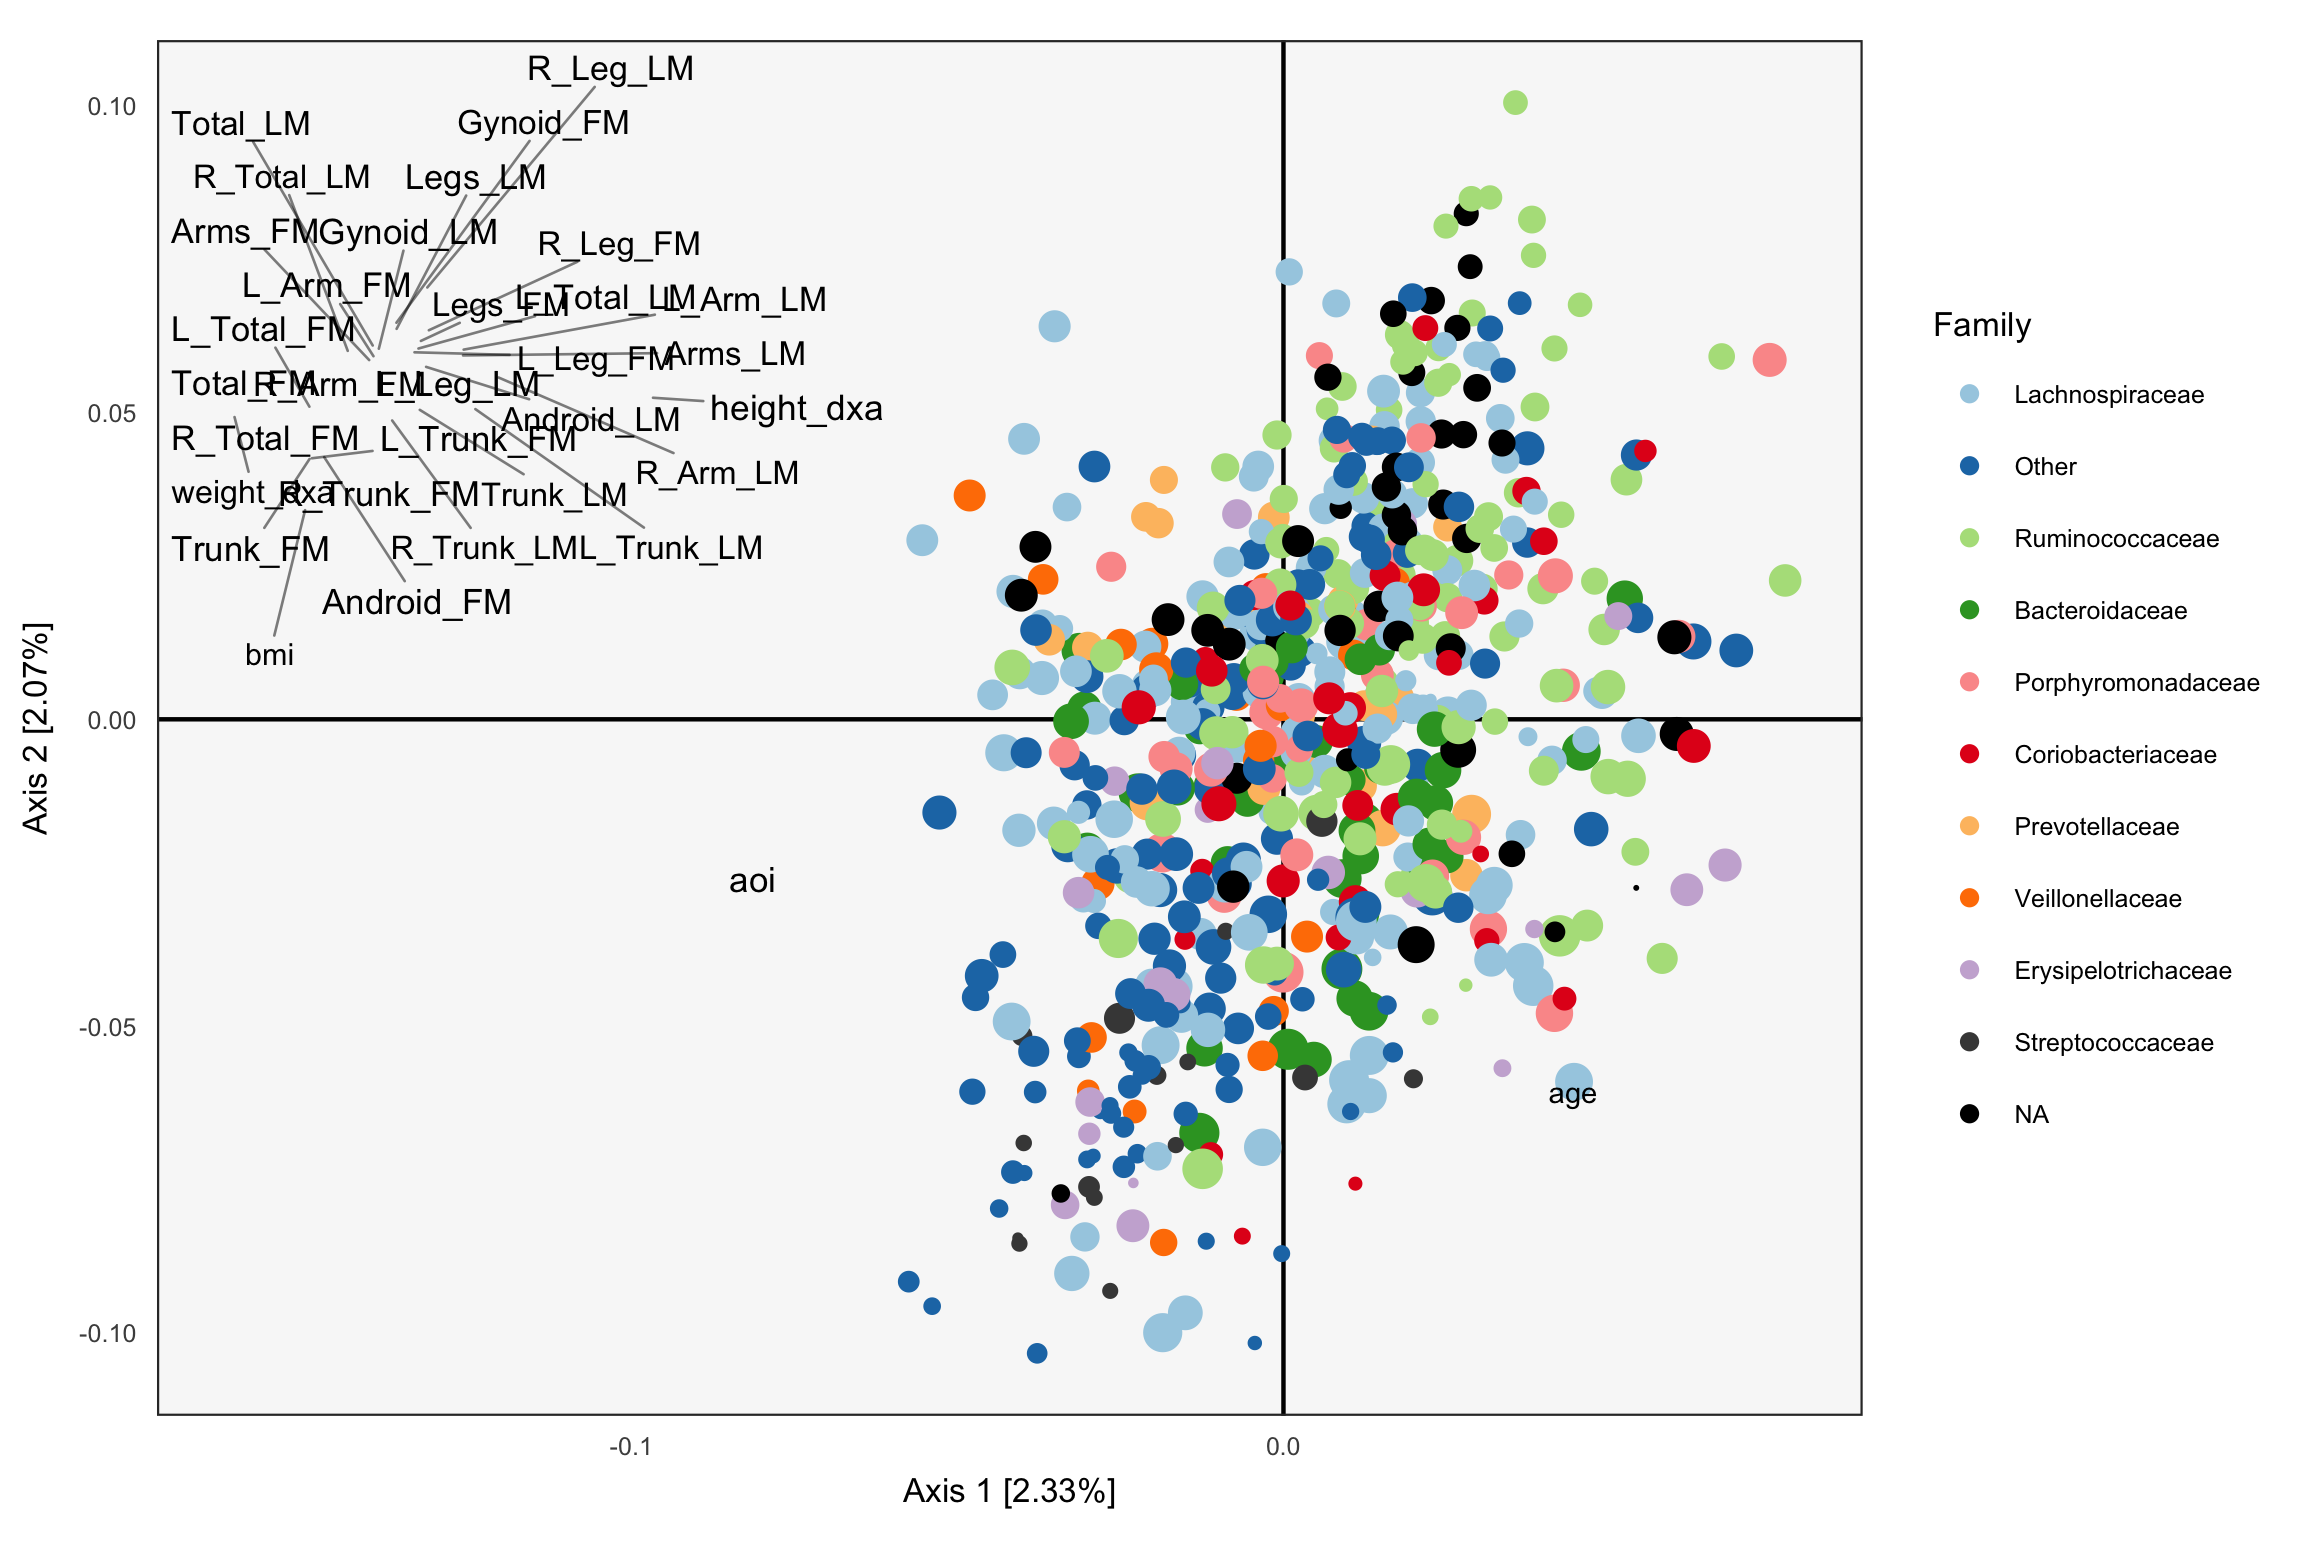
\includegraphics[width=0.47\textwidth]{figure/pca_loadings}
    \caption{The simplest multitable approach is to merge tables. Here we use
      PCA, treating taxa as rows, so that the usual covariance matrix estimator
      is well defined. We have used an rlog transform of species abundances, and
      centered / scaled both tables. \label{fig:pca_multitable}}
  \end{figure}
\end{frame}

\subsection{CCA}
\label{subsec:CCA}

\begin{frame}
  \frametitle{Canonical Correlation Analysis (CCA)}
\begin{itemize}
\item The PCA approach ignores the fact that different sets of columns come from
  different tables
\item In contrast, CCA directly identifies directions maximizing
  covariation across tables. The first directions $u$ and $v$ are chosen as
  optimal values in
\begin{align*}
  \text{maximize}_{u \in \reals^{p_{1}}, v \in \reals^{p_{2}}}
  &u^{T}\hat{\Sigma}_{XY}v \\
  \text{subject to } & u^{T}\hat{\Sigma}_{XX}u = 1 \nonumber \\
  & v^{T}\hat{\Sigma}_{YY}v = 1. \nonumber
\end{align*}
\end{itemize}
\end{frame}

\begin{frame}
  \frametitle{CCA}
  \begin{figure}[ht]
    \centering
    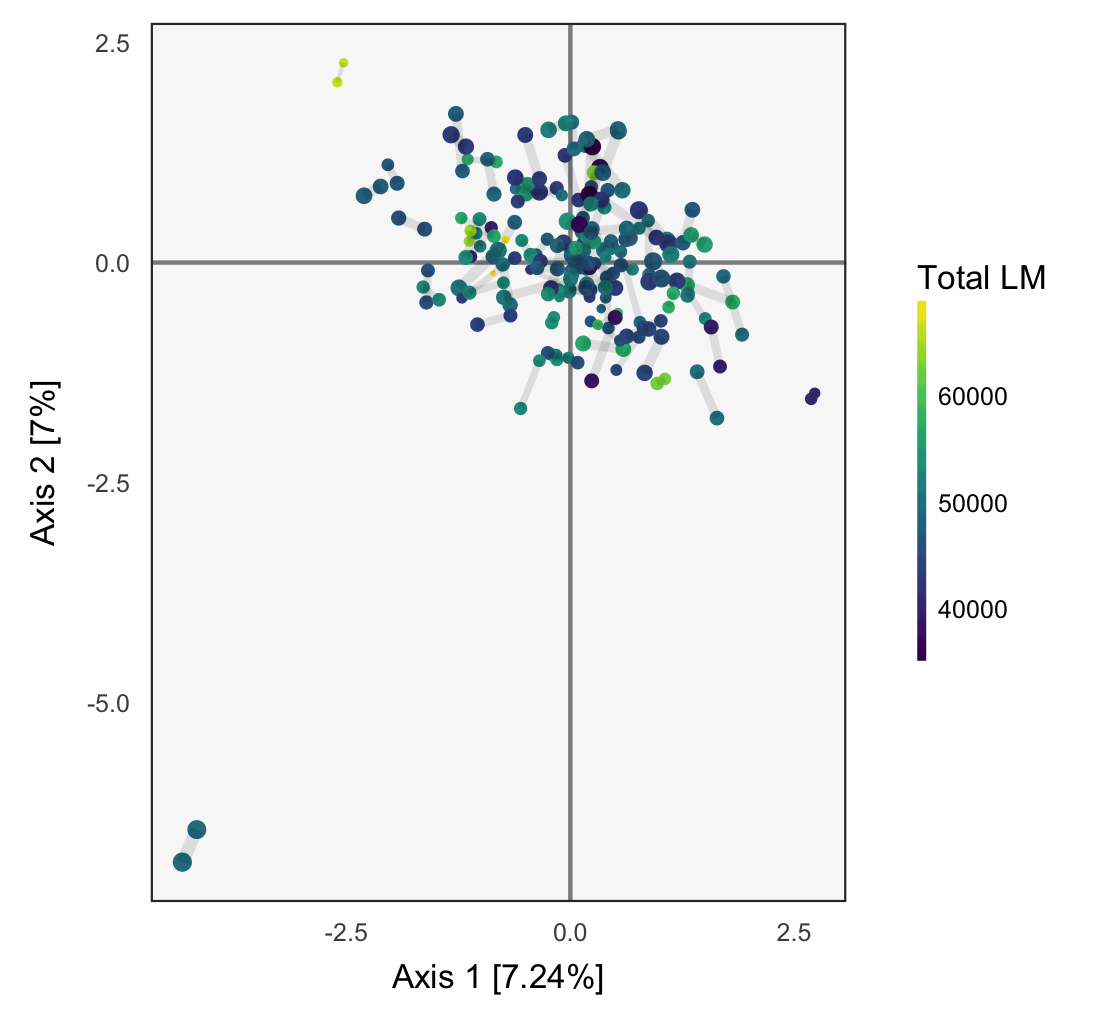
\includegraphics[width=0.45\textwidth]{figure/cca_scores_lm}
    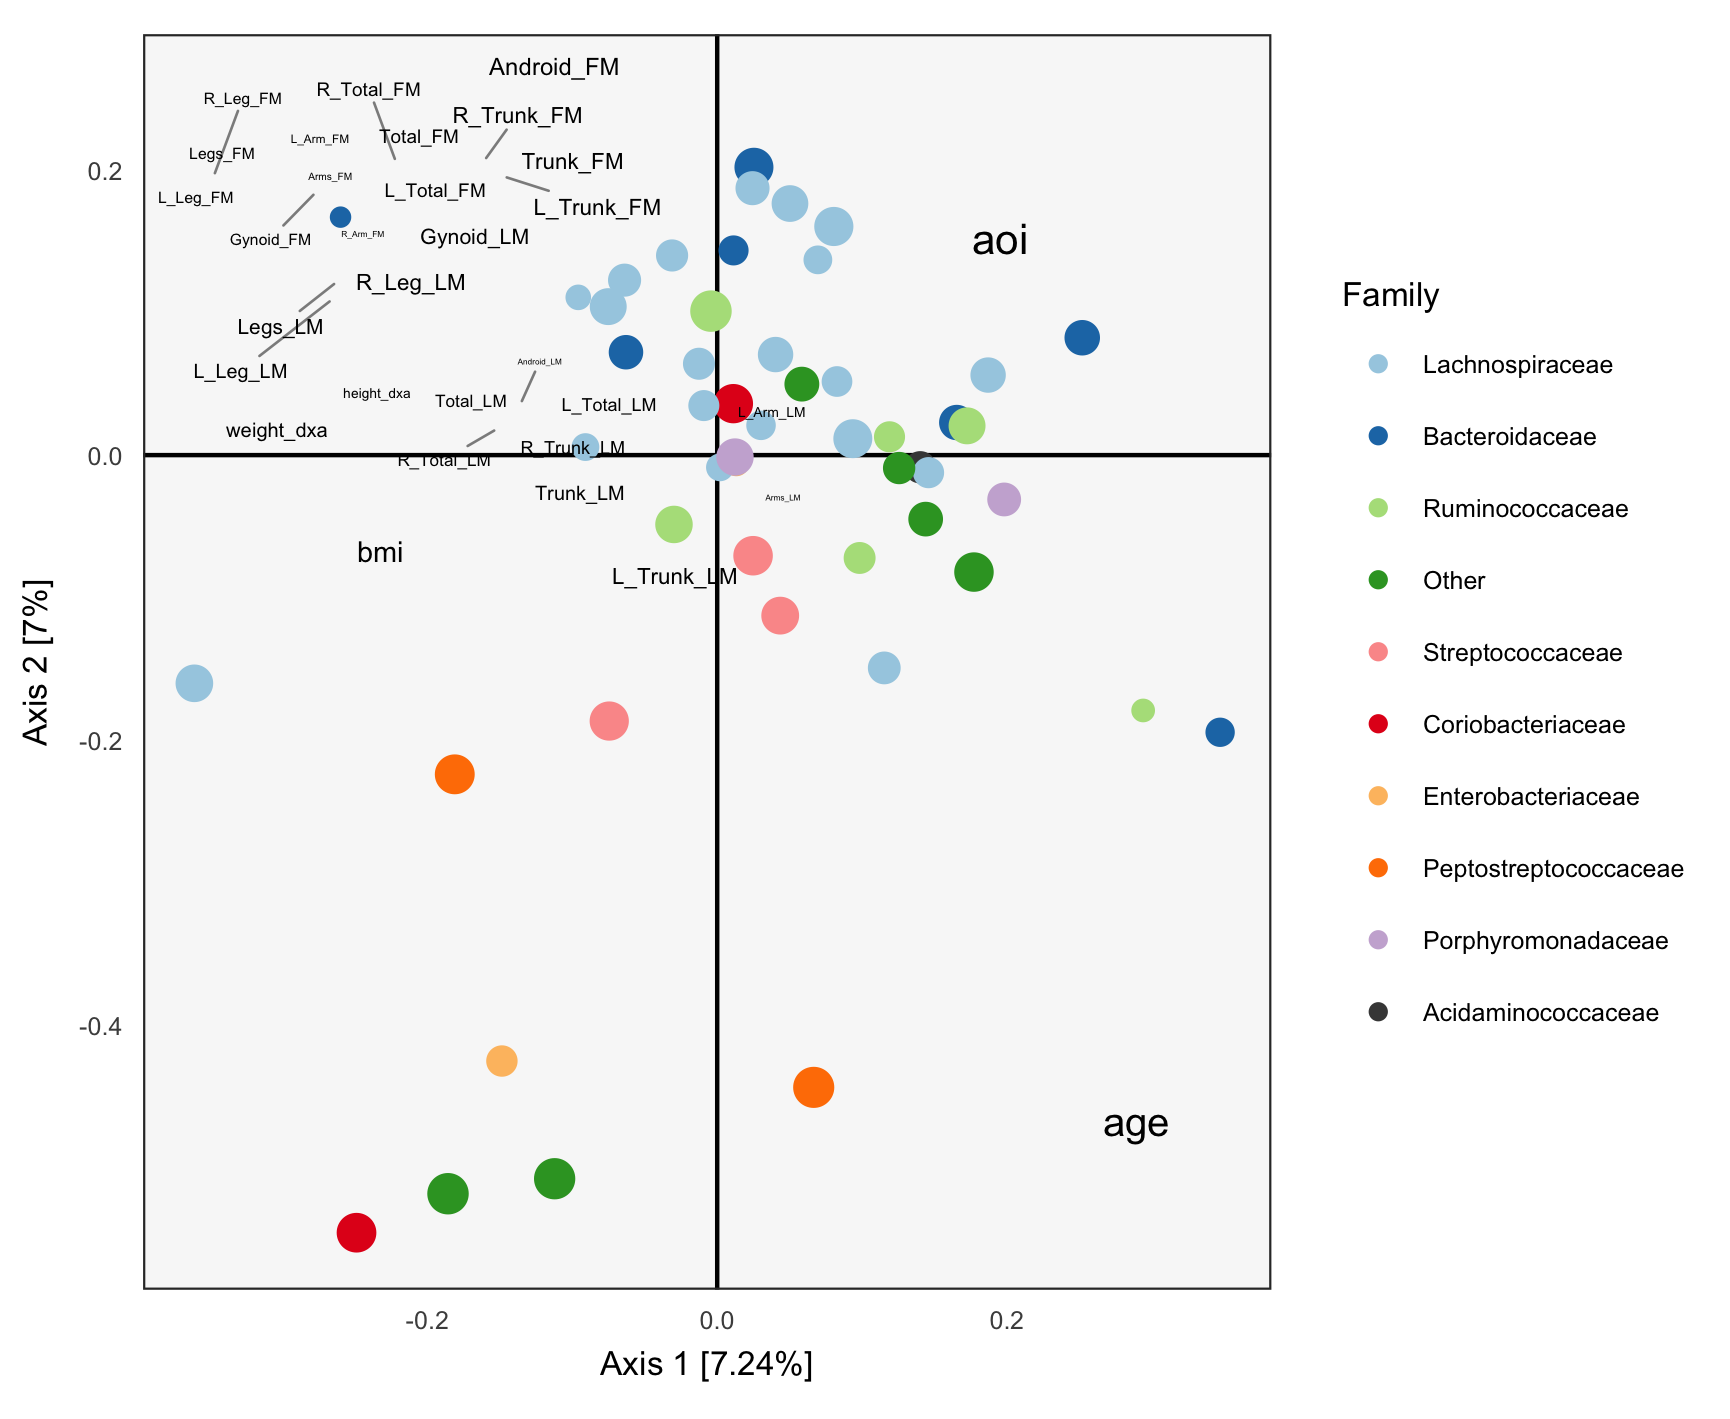
\includegraphics[width=0.47\textwidth]{figure/cca_loadings}
    \caption{We subset to 51 species using a $k$-over-$0$ filter, since
      otherwise covariance estimation is poorly defined.
      \label{fig:cca_scores}}
  \end{figure}
\end{frame}

\subsection{Sparse CCA}
\label{subsec:sparse_cca}

\begin{frame}
  \frametitle{Sparse CCA}
  \begin{itemize}
  \item For high-dimensional situations, many regularized versions of CCA have
    been developed \citep{zou2006sparse, witten2009penalized, hardoon2011sparse,
      balakrishnan2012sparse}
  \item We focus on the formulation of \citep{witten2009penalized},
    \begin{align*}
  \text{maximize}_{c_{1}^{(1)} \in \reals^{p_{1}}, c_{1}^{(2)} \in
    \reals^{p_{2}}} & c_{1}^{(1) T}\hat{\Sigma}_{12}
  c_{1}^{(2)} \\
  \text{subject to } &\|c_{1}^{(1)}\|_{2}^{2} = \|c_{1}^{(2)}\|_{2}^{2} = 1 \\
  &\|c_{1}^{(1)}\|_{1} \leq \mu_{1} \\
  &\|c_{1}^{(2)}\|_{1} \leq \mu_{2}
    \end{align*}
  \end{itemize}
\end{frame}

\begin{frame}
  \frametitle{Sparse CCA}
  \begin{figure}[ht]
    \centering
    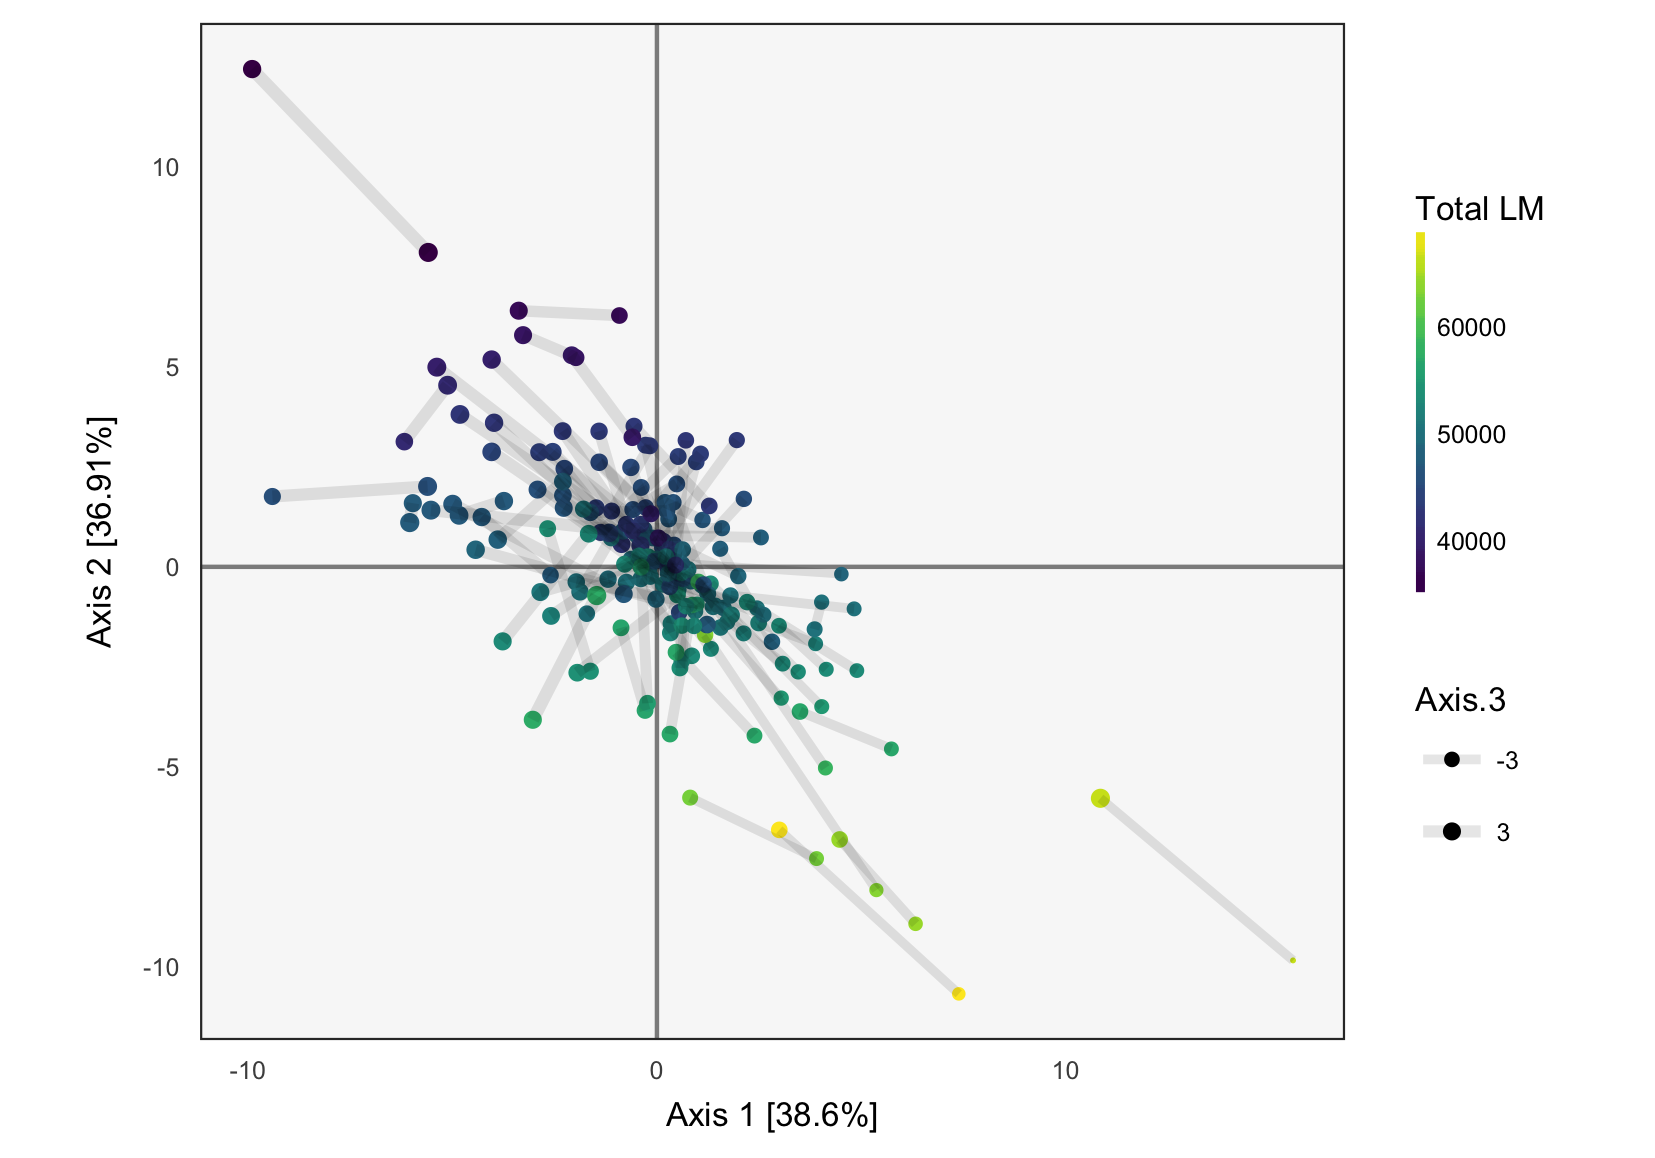
\includegraphics[width=0.45\textwidth]{figure/pmd_scores_lm}
    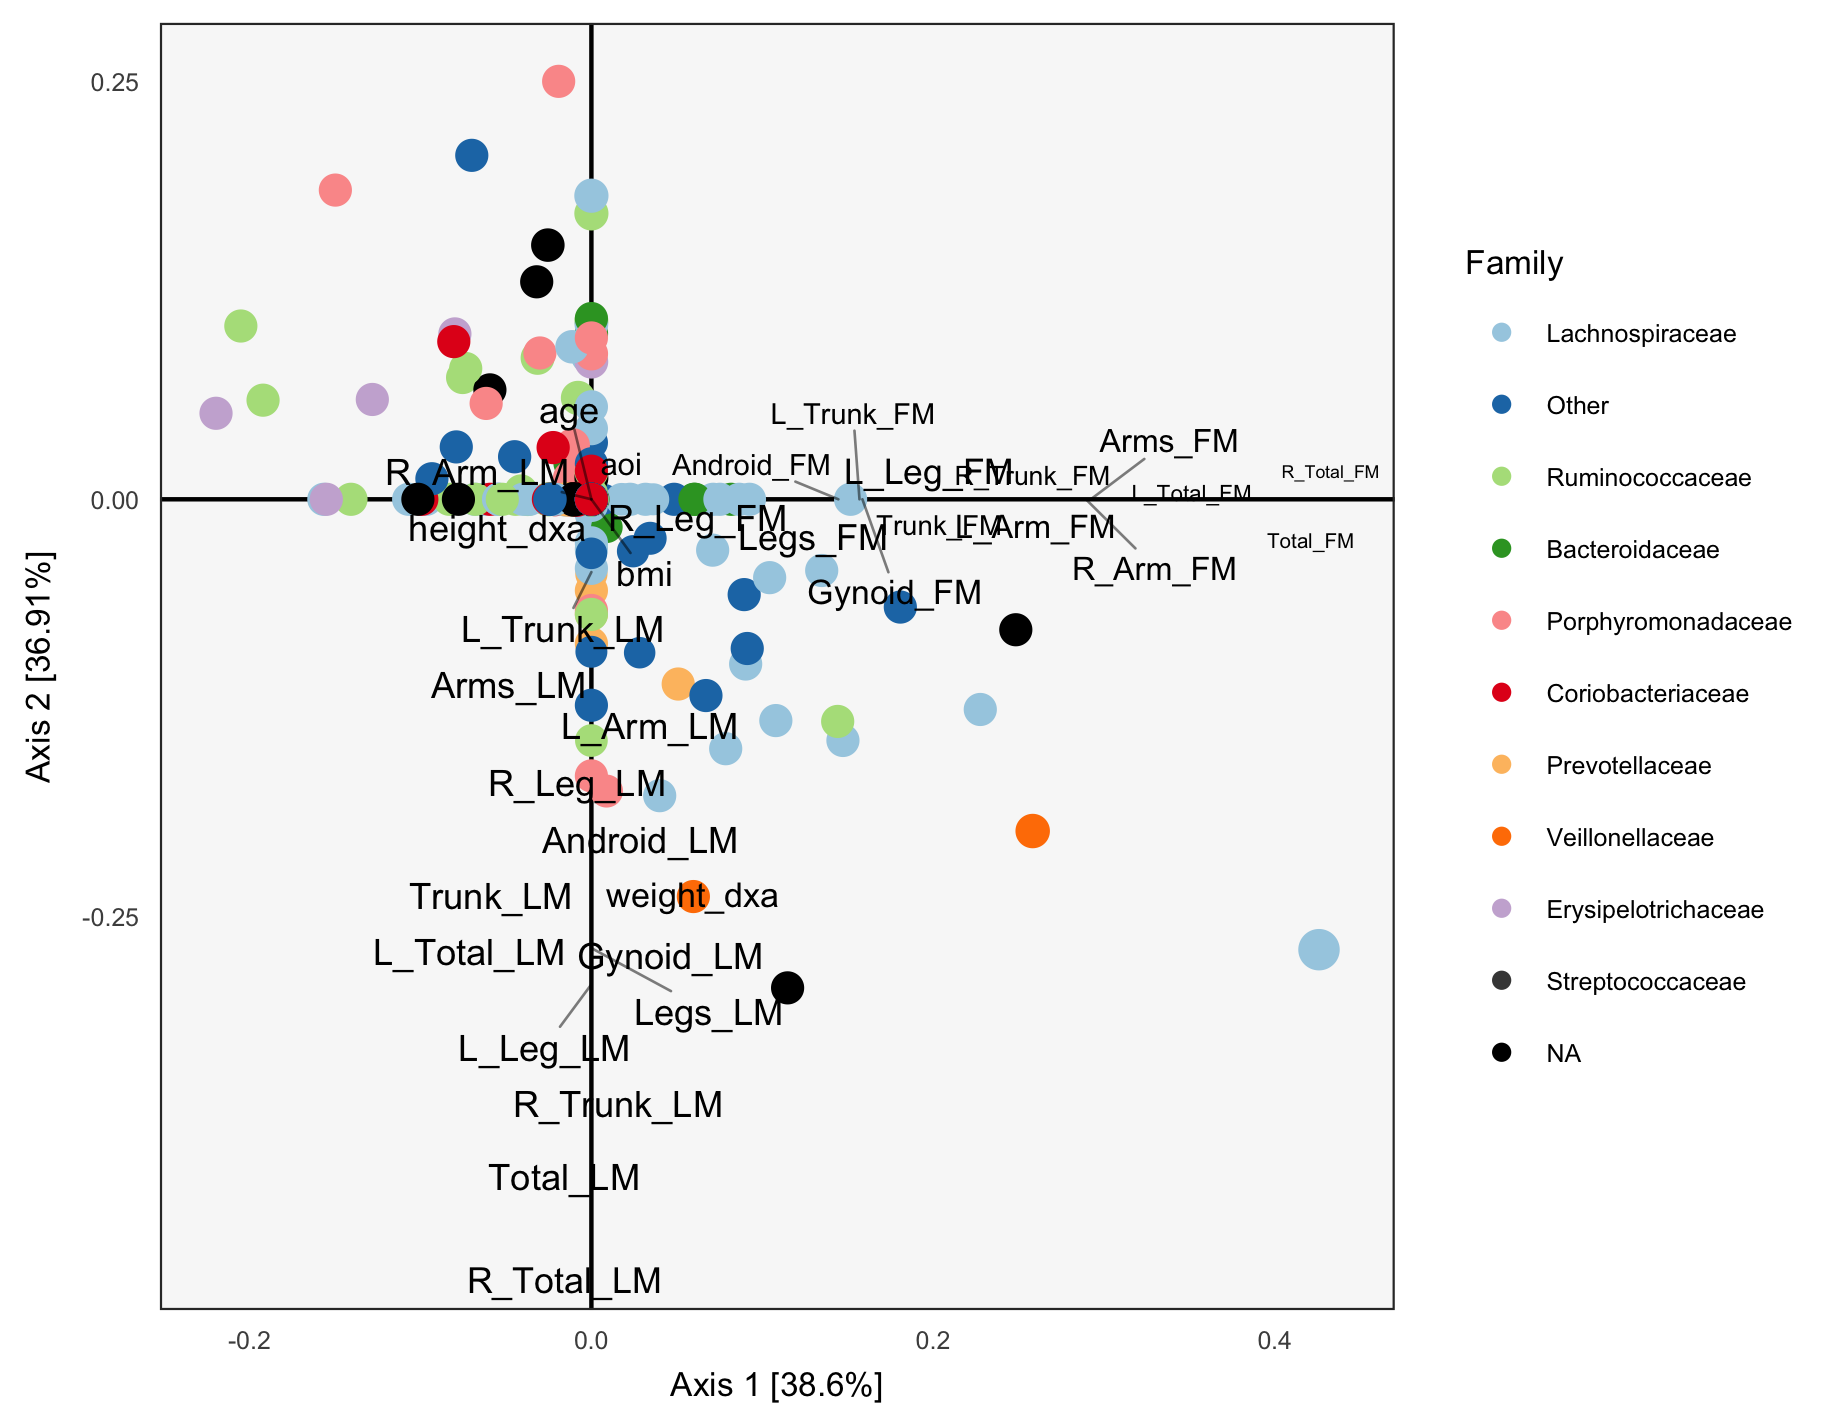
\includegraphics[width=0.47\textwidth]{figure/pmd_loadings}
    \caption{We no longer have to subset taxa, since we are regularizing the CCA
      optimization. There does seem to be meaningful covariation across tables,
      and the top two CCA correlations are a little over
      0.7. \label{fig:pmd_scores}}
  \end{figure}
\end{frame}

\subsection{CCA / LDA}
\label{subsec:cca_lda}

\begin{frame}
  \frametitle{CCA / LDA}
  \begin{itemize}
  \item There is a probabilistic interpretation of CCA in terms of shared scores
    in a pair of factor analysis models \citep{bach2005probabilistic}
  \item We consider a slight modification for the case when one table is counts
  \item We could use exponential family PCA, NMF, but for concreteness consider LDA,
    \begin{align*}
      y_{i} \vert \xi_{i}^{s}, \xi^{y} &\sim \Gsn\left(y_{i} \vert W^{Y}\xi_{i}^{s} +
      B^{Y}\xi_{i}^{y} + \mu_{Y}, I_{d}\right) \\
      x_{i} \vert \xi_{i}^{s}, \xi_{i}^{x} &\sim \Mult\left(x_{i} \vert N_{i},
      \mathcal{S}\left(B^{X} \xi_{i}^{s} + W^{X} \xi_{i}^{x}\right)\right) \\
      \xi_{i}^{\cdot} &\sim \Gsn\left(0, \tau_{\cdot}^{2}\right)
    \end{align*}
    where $\left[\mathcal{S}\left(v\right)\right]_{k} =
    \frac{\exp{v_{k}}}{\sum_{k^{\prime}}\exp{v_{k^{\prime}}}}$ is the softmax.
  \end{itemize}
\end{frame}

\begin{frame}
  \frametitle{(Within) Body Composition Loadings}
\begin{figure}[ht]
  \centering
  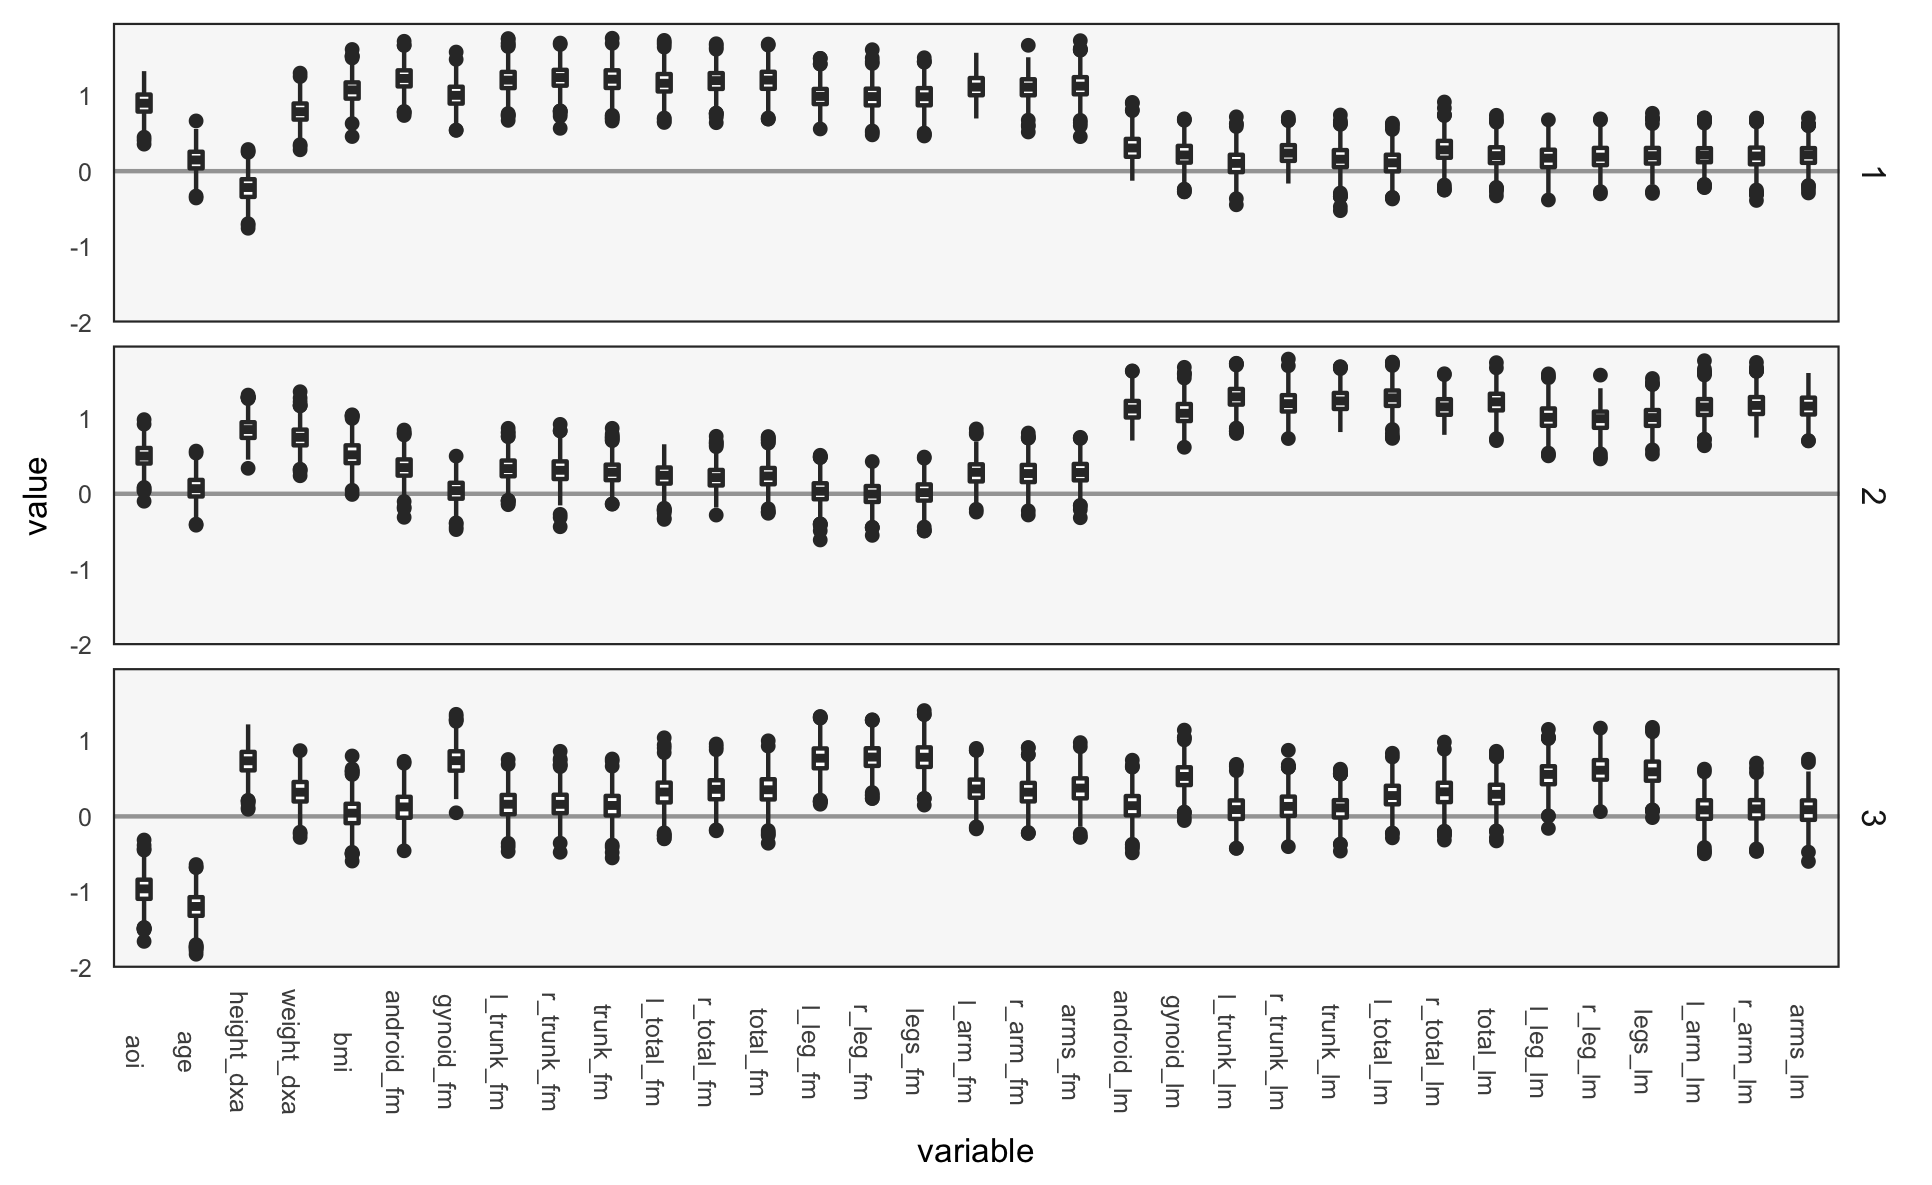
\includegraphics[width=0.7\textwidth]{figure/within_loadings_body_comp_boxplots}
  \caption{Posterior for $W^{Y}$, the body-composition table specific loadings.
    Each row corresponds to one factor, and each boxplot corresponds to one
    variable in that factor.\label{fig:within_loadings_body_comp_boxplots} }
\end{figure}
\end{frame}

\begin{frame}
  \frametitle{(Within) Body Composition Scores}
 \begin{figure}[ht]
   \centering
   
\includegraphics[width=0.9\textwidth]{figure/unshared_scores_lm_posterior}
   \caption{Posterior samples of scores $\xi^{Y}_i$ associated with the body
     composition variables. These are much more spread out than those for
     species. \label{fig:unshared_scores_lm_posterior} }
 \end{figure}
\end{frame}

\begin{frame}
  \frametitle{(Within) Species Loadings}
\begin{figure}[ht]
  \centering
  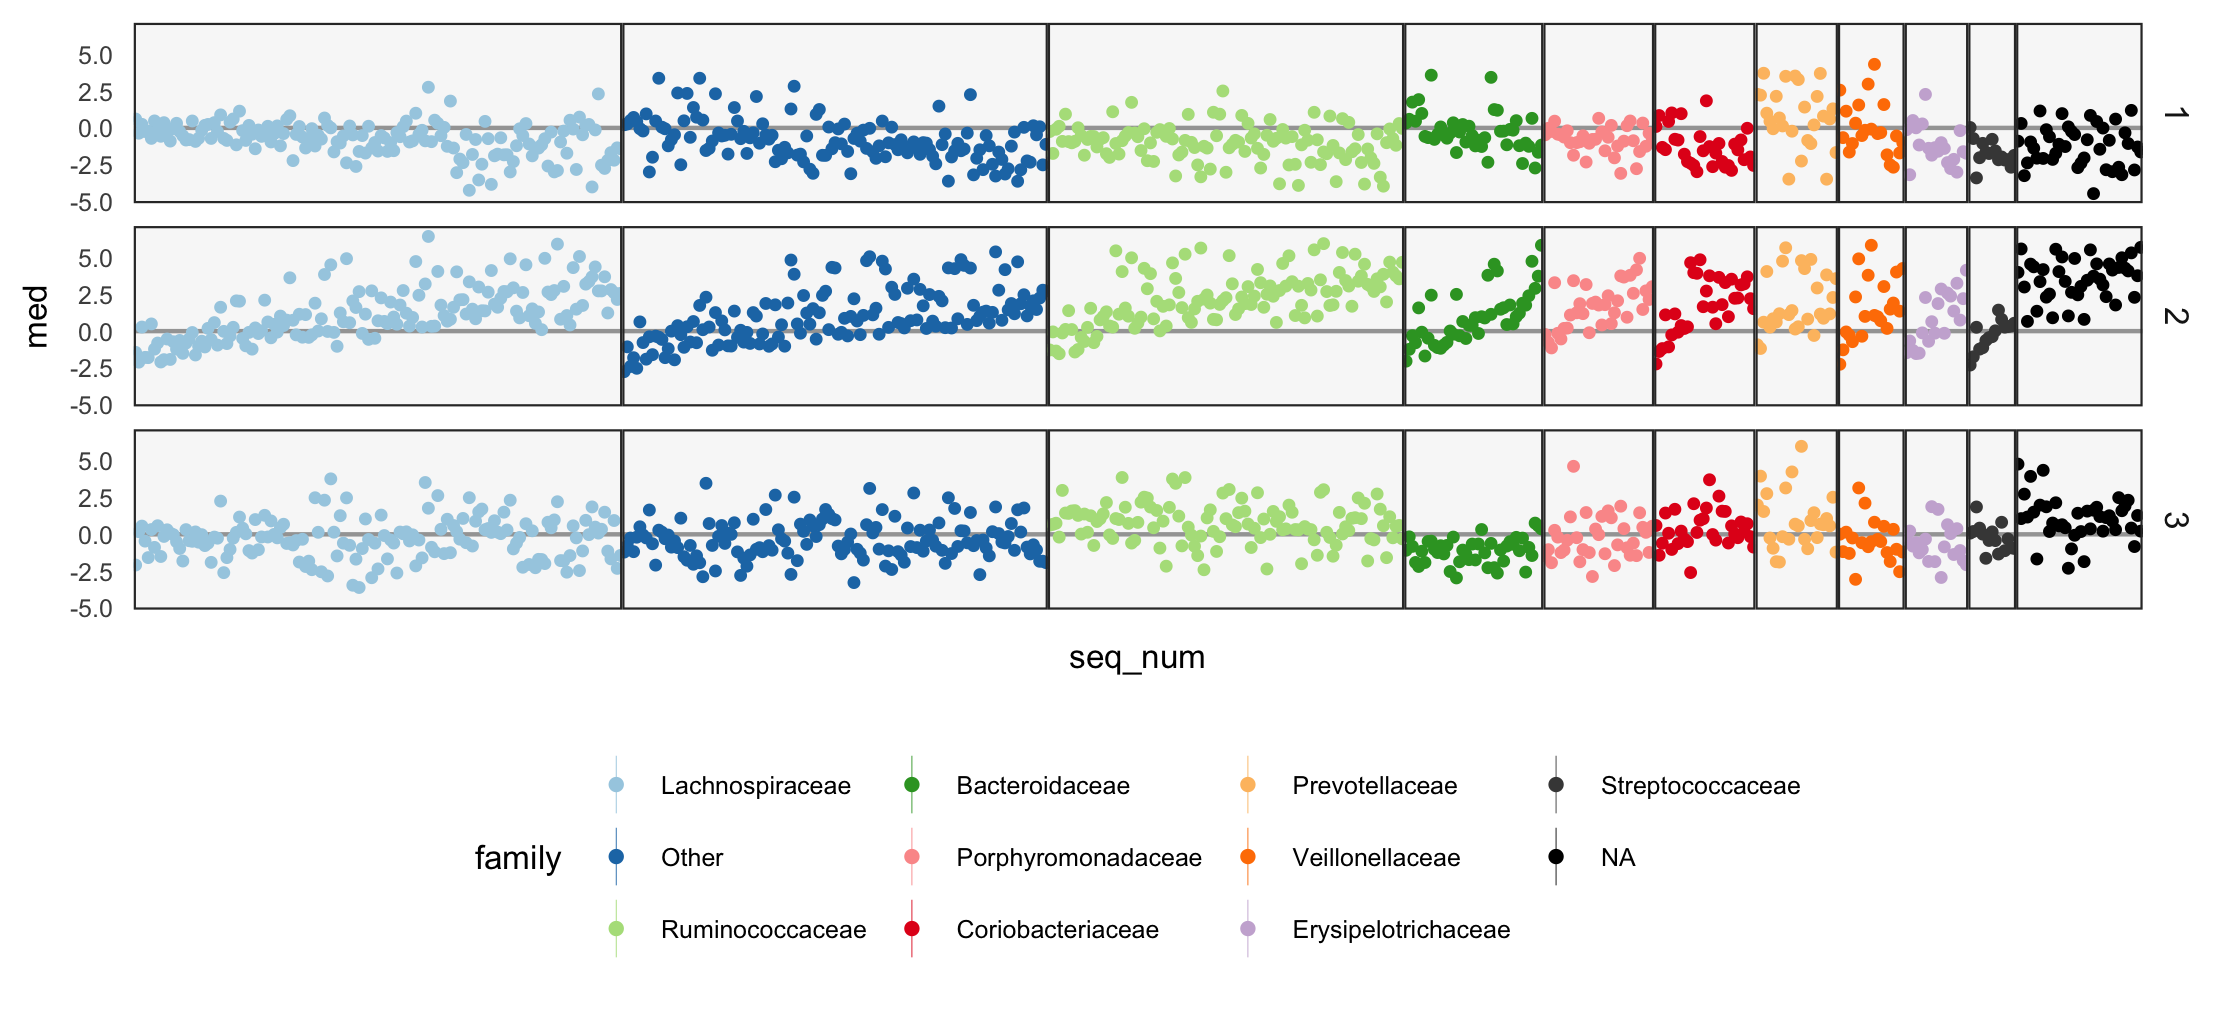
\includegraphics[width=\textwidth]{figure/within_loadings_seq_boxplots}
  \caption{The analog of Figure \ref{fig:within_loadings_body_comp_boxplots},
    but for the species loadings
    instead. Be careful that these loadings could be reflected or rotated
    without affecting the likelihood. \label{fig:within_loadings_seq_boxplots} }
\end{figure}
\end{frame}

\begin{frame}
  \frametitle{(Between) Body Composition Loadings}
\begin{figure}[ht]
  \centering
  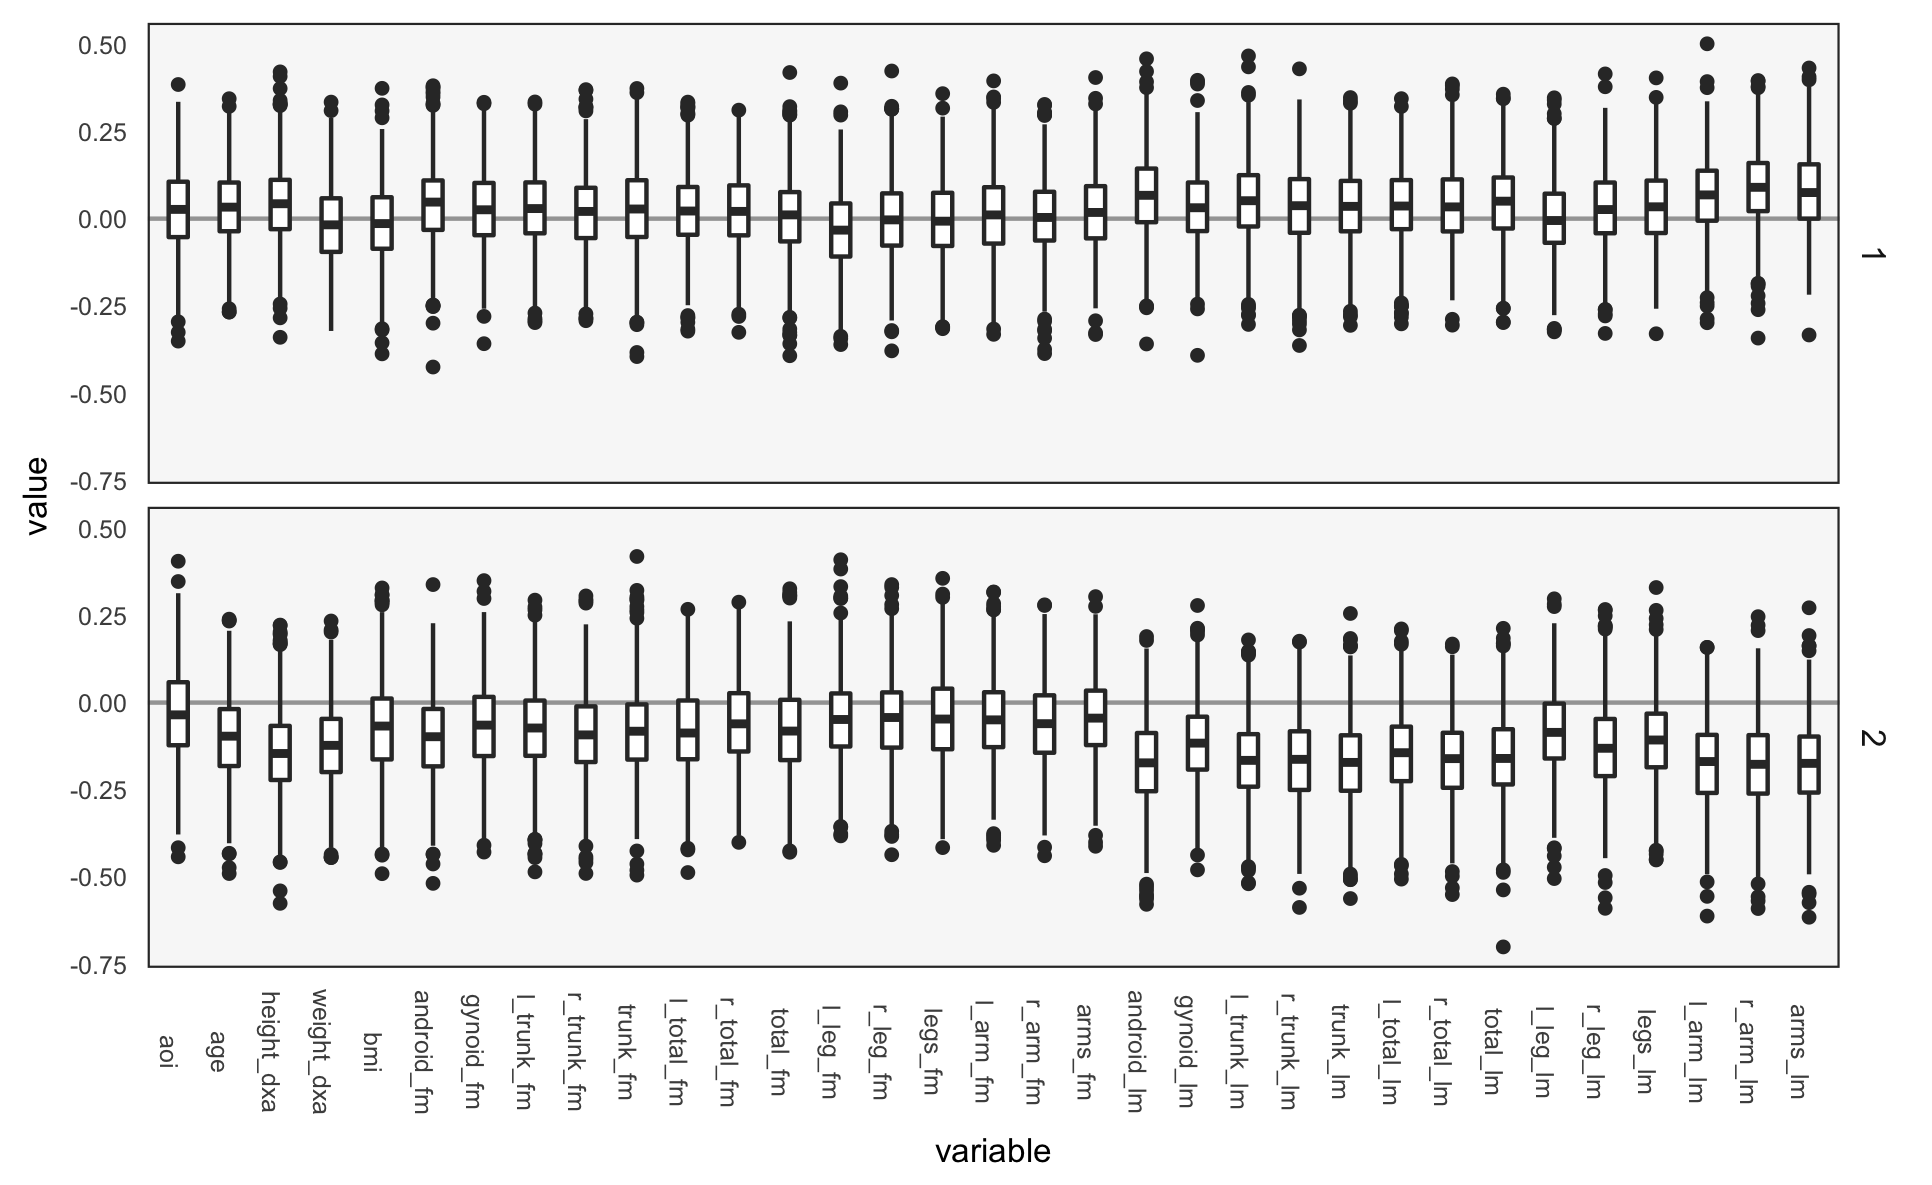
\includegraphics[width=0.75\textwidth]{figure/between_loadings_body_comp_boxplots}
  \caption{The analog of Figure \ref{fig:within_loadings_body_comp_boxplots} for
    loadings associated with \texttt{shared} scores, which is of primary
    interest when studying covariation across
    tables. \label{fig:shared_loadings_body_comp_boxplots} }
\end{figure}
\end{frame}

\begin{frame}
  \frametitle{(Between) Species Loadings}
  \begin{figure}[ht]
    \centering
    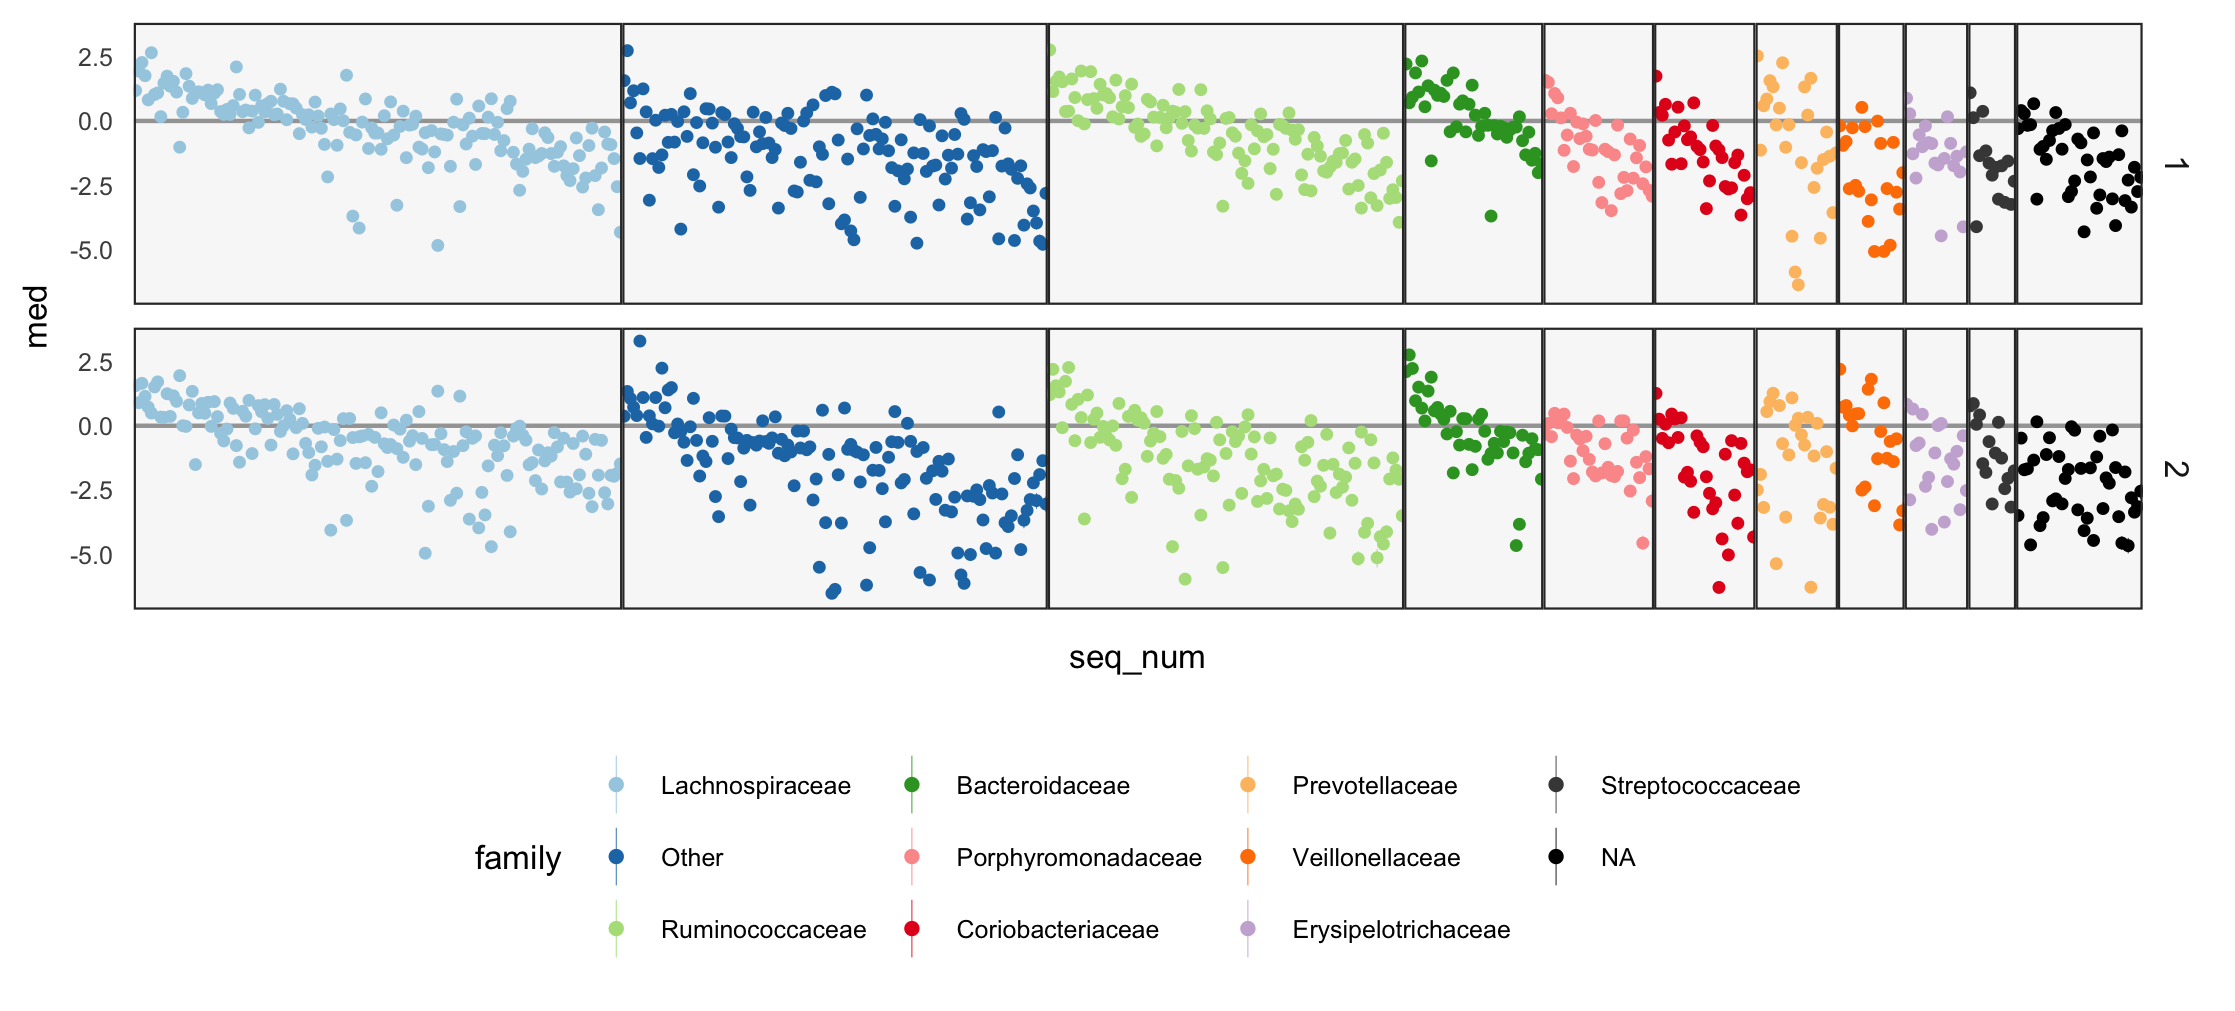
\includegraphics[width=\textwidth]{figure/between_loadings_seq_boxplots}
    \caption{The analog of Figure \ref{fig:within_loadings_seq_boxplots} for
      species abundances. \label{fig:shared_loadings_seq_boxplots} }
  \end{figure}
\end{frame}

\begin{frame}
  \frametitle{Conclusion}
  \begin{itemize}
  \item Potential directions for improvement,
    \begin{itemize}
    \item Sharing information between sequences in scan sampling and mixture of GPs?
    \item BASIC model with more plausible likelihood model, when abundances have long tail?
    \item Posterior checks, improved priors, and quantitative tuning for
      probabilistic approaches?
    \item Incorporating all $\sim 2000$ individuals available for body
      composition clustering?
    \end{itemize}
  \end{itemize}
\end{frame}

\bibliographystyle{plainnat}
\bibliography{refs.bib}

\section{Appendix}
\label{sec:Appendix}

\begin{frame}
  \frametitle{PCA-IV}
\begin{figure}
  \centering
  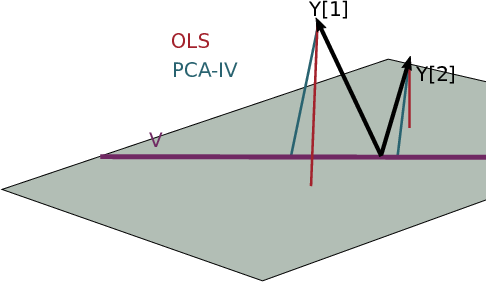
\includegraphics[width=0.7\textwidth]{figure/pca_iv_geometry}
  \caption{A geometric view of PCA-IV. The columns of the response $Y$ are views
    as $n$-dimensional vectors. The grey plane is the span of
    $X$. Multivariate OLS simply projects the columns of $Y$ onto the plane,
    while PCA-IV searches for a further subspace $V$ on which to project all
    responses. \label{fig:pca_iv_geometry} }
\end{figure}
\end{frame}

\begin{frame}
  \frametitle{PCA-IV}
    \begin{figure}[ht]
      \centering
      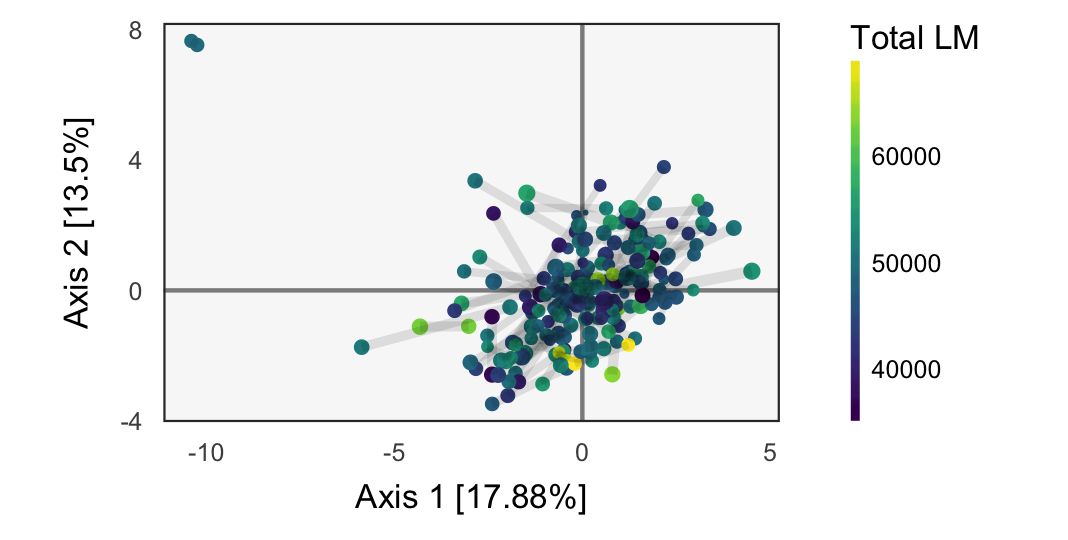
\includegraphics[width=0.48\textwidth]{figure/pcaiv_scores_total_lm}
      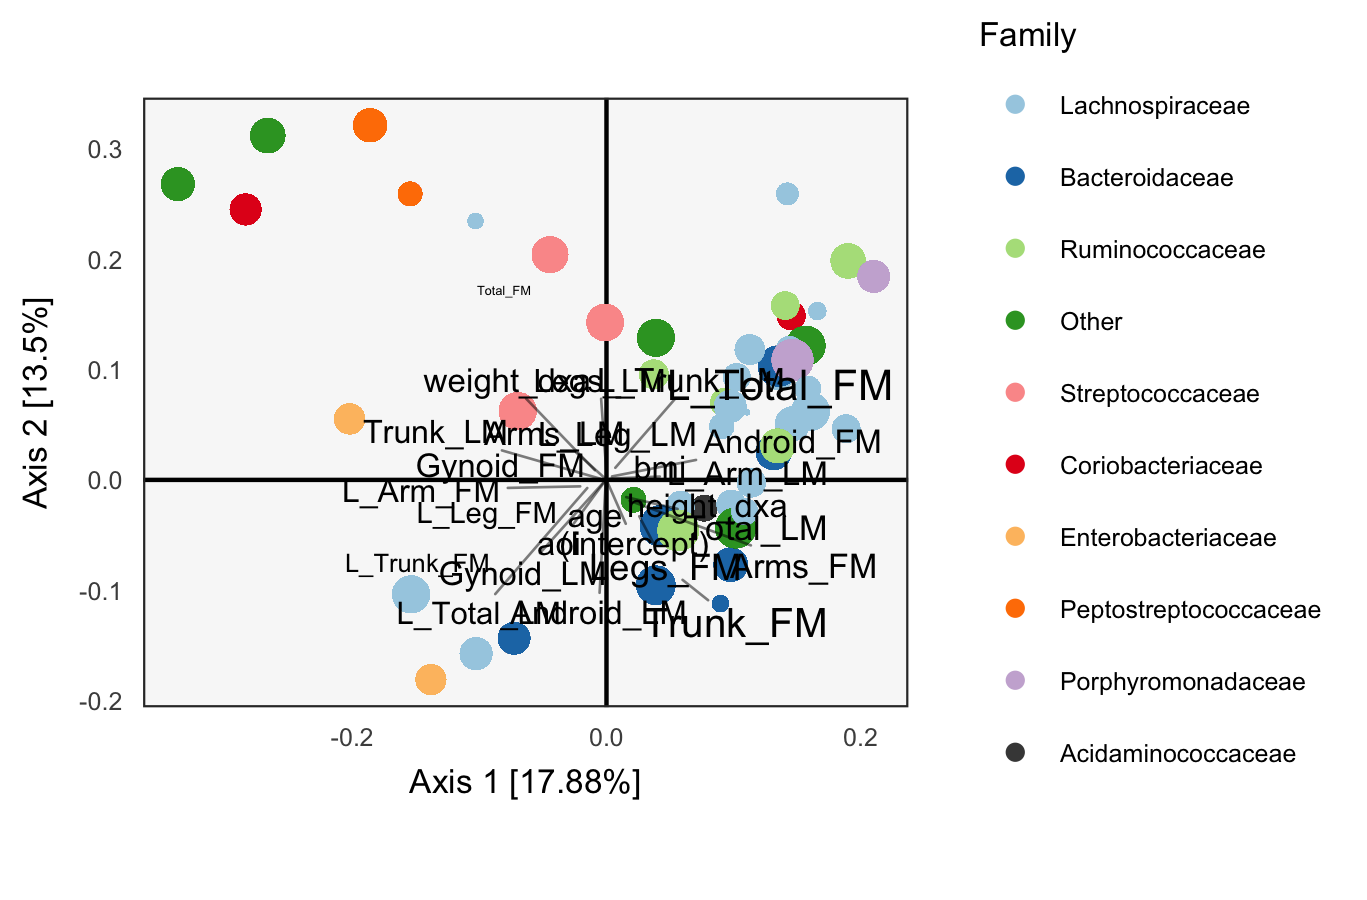
\includegraphics[width=0.45\textwidth]{figure/pcaiv_loadings}
      \caption{The results of PCA-IV on the WELL-China
        data. \label{fig:pcaiv_scores_loadings} }
    \end{figure}
\end{frame}

\begin{frame}
  \frametitle{Canonical Correspondence Analysis}
  \begin{itemize}
  \item Come up with scores for species and for sites ($z_{i}$ and $q_{j}$)
  \item Scores for different sites should be a weighted average of the species
    scores, with larger weights for the species that are more common at those
    sites.
    \begin{align*}
      z_{i} \propto \frac{1}{f_{i\cdot}}\sum_{j = 1}^{p_{1}}f_{ij}q_{ij} \\
      q_{j} \propto \frac{1}{f_{\cdot j}} \sum_{i = 1}^{n} f_{ij}z_{ij},
    \end{align*}
  \item Projecting $Q$ onto the span of site characteristics between iterations
    gives canonical correspondence analysis
  \end{itemize}  
\end{frame}

\begin{frame}
  \frametitle{Canonical Correspondence Analysis}
\begin{figure}[ht]
  \centering
  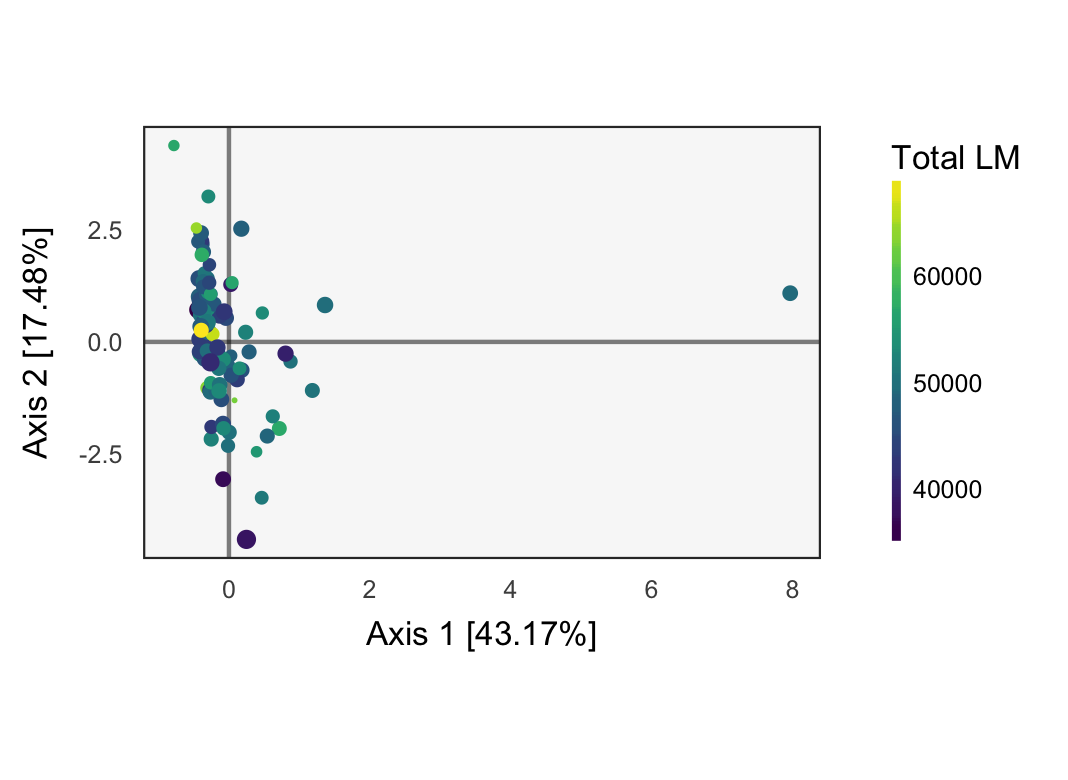
\includegraphics[width=0.48\textwidth]{figure/ccpna_scores_total_lm}
  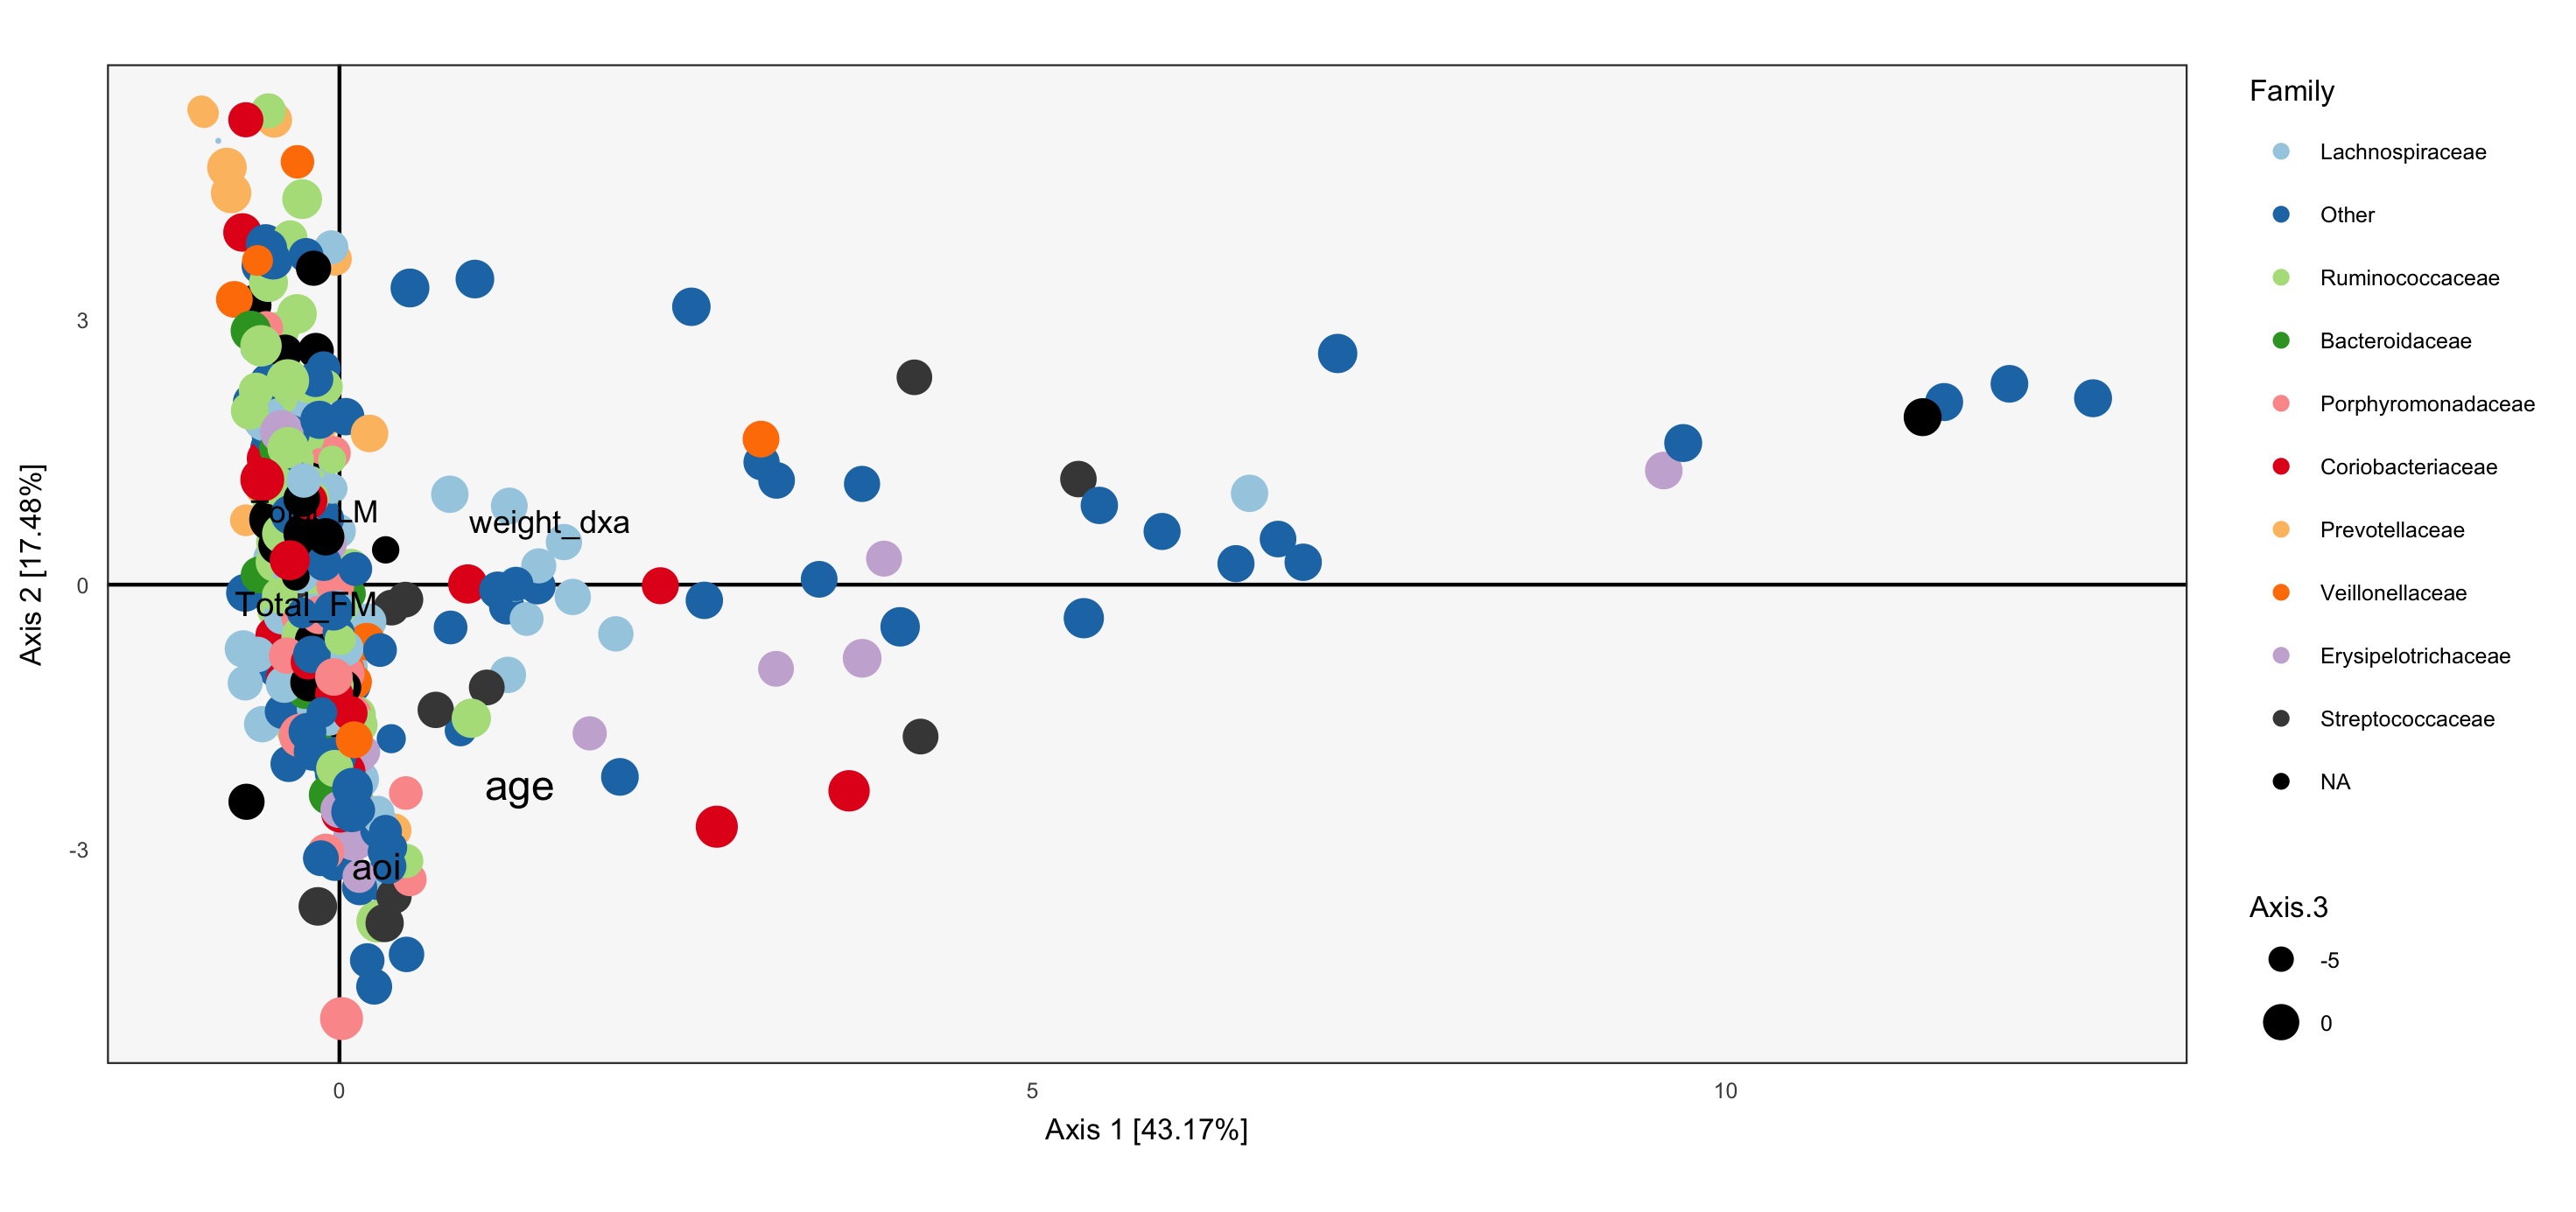
\includegraphics[width=0.45\textwidth]{figure/ccpna_loadings}
  \caption{The results of canonical correspondence analysis on the WELL-China
    data.\label{fig:ccpna_scores_loadings} }
\end{figure}
\end{frame}


\end{document}
